% Working revision for Telecommunication Systems. Review before submission.
\documentclass[pdflatex,iicol,sn-mathphys-num]{sn-jnl}
\usepackage{amsmath,amssymb,amsthm,booktabs,graphicx,tabularx}
\usepackage{xurl}
\emergencystretch=2em
\theoremstyle{thmstyleone}
\newtheorem{proposition}{Proposition}
\newtheorem{lemma}{Lemma}
\raggedbottom
\begin{document}
\title[Robust Spacetime Compliance in Vehicular Crowdsensing]{Zero-Knowledge Certification of Robust Spacetime Compliance under Byzantine Evidence for Vehicular Crowdsensing}
\author[1]{\fnm{Lili} \sur{He}}
\author[1]{\fnm{Sheng} \sur{Jiang}}
\author[1]{\fnm{Shuang} \sur{Chen}}
\author*[1]{\fnm{Lei} \sur{Zhang}}\email{8213662@163.com}
\affil[1]{\orgdiv{College of Information and Electronic Technology}, \orgname{Jiamusi University}, \orgaddress{\city{Jiamusi}, \postcode{154007}, \country{China}}}
\abstract{In vehicular crowdsensing, a location-privacy mechanism may need to establish compliance with a spatial policy without revealing a vehicle's coordinates. Yet positioning errors, environmental effects, and synchronization uncertainty often leave only interval-valued spacetime observations. Even authenticated sources may share systematic bias or behave in a Byzantine manner. We propose a privacy-preserving compliance certification method based on signed spacetime uncertainty evidence. Given an upper bound $f$ on Byzantine issuers and an allowance $r$ for honest issuers whose intervals miss the true event, the method constructs the feasible set of states supported by at least $k = n - f - r$ issuers. A report is accepted only when this set is nonempty and wholly contained in the authorized region. The resulting decision distinguishes valid, invalid, ambiguous, and inconsistent evidence. We implement two Groth16/BN254 circuits that verify elliptic-curve digital signatures with the MiMC hash and bind the proof to the task, issuer roster, report, threshold, challenge nonce, and expiry. Gateway tests reject tampering, context substitution, expired challenges, and cross-challenge replay; only one of eight concurrent copies of a valid request is accepted within a single gateway instance. Across 12 synthetic conditions satisfying the configured fault and coverage assumptions, mean decisive coverage is 87.52\%, compared with 75.63\% for a fixed-margin baseline. Tested subset circuits produce 164-byte proofs with median proving times of 163--255 ms on an Apple M1. The certification layer leaves issuer enrollment and sensor calibration to the surrounding vehicular crowdsensing platform.}
\keywords{Zero-knowledge proofs, Location privacy, Vehicular crowdsensing, Byzantine evidence, Robust evidence fusion, Spacetime compliance certification}
\maketitle

\section{Introduction}
In location-privacy applications, a verifier may need to establish that a user satisfies a spatial policy without learning the user's precise coordinates. Zero-knowledge location proofs, for example, can verify membership in a designated region while keeping the location private ~\citep{ZKLP,VehiclePolicy}. Such verification commonly starts from a definite spacetime position. Vehicle sensing, however, cannot always provide an observation of that kind. Positioning error, environmental interference, and clock-synchronization uncertainty may restrict the available evidence to a range of plausible positions and times. A valid source signature authenticates the evidence submitted by that source; it does not establish that the physical estimate is accurate. Compromised sources may also sign deliberately misleading observations. Consequently, even a mathematically correct proof concerning a hidden coordinate does not establish that the chosen coordinate is sufficiently supported by observations. This paper asks how multiple uncertain, and potentially malicious, spacetime observations can support a policy-compliance claim without being disclosed to the verifier.

The problem is particularly relevant to vehicular crowdsensing. Distributed vehicle observations support traffic monitoring, road management, and environmental-sensing tasks ~\citep{Suhag2023,Zheng2025BARM}, for which the admissibility of a report may depend on the event's location and time. Revealing the positioning evidence can expose a vehicle's mobility history. Replacing several interval-valued observations with one representative point, however, can conceal disagreement near a policy boundary. Requiring every source interval to intersect is not necessarily safer: a Byzantine issuer may submit a displaced interval that excludes the true state while leaving a small intersection entirely within the authorized region. A sound compliance rule therefore needs to specify which possible states have sufficient evidential support and how conflicting observations are handled, in addition to protecting those observations.

We consider privacy-preserving compliance certification over signed spacetime uncertainty evidence. Each enrolled issuer signs an axis-aligned integer box for the same reference event. For $n$ issuers, at most $f$ Byzantine sources, and at most $r$ honest observations that fail to cover the true state, let $k = n - f - r$. The robust feasible set $\mathcal{F}_k$ consists of the states covered by at least $k$ signed boxes. Compliance is certified only if this set is nonempty and entirely contained in the authorized policy. A nonempty feasible set lying outside the policy produces an invalid decision; a set crossing the boundary is ambiguous; and a set with no threshold-supported state is inconsistent. A valid decision is reserved for the acceptance condition. These four outcomes avoid treating an arbitrarily chosen point as conclusive and distinguish a conflict in otherwise valid evidence from failure to submit the required evidence.

The support-depth construction follows classical fault-tolerant interval fusion, including Marzullo's threshold-intersection principle. Here we develop an exact zero-knowledge certification of that construction and a report-bound gateway to enforce it.

We combine threshold-based fault-tolerant interval reasoning ~\citep{Marzullo1990,BFTPoLoc,PG,CRSF} with zero-knowledge certification. Rather than revealing the source intervals, the prover establishes that the signatures satisfy the roster and context constraints and that the reported decision follows from the same threshold rule. A report-binding protocol associates this proof with the task, issuer roster, report bytes, threshold, challenge nonce, and expiry. This association prevents a proof for one authorized context from being reused as evidence for another, under the stated cryptographic and gateway assumptions.

In a conventional gateway-side fusion design, submitting each signed uncertainty box to the verifier would reveal sensitive spatiotemporal positioning envelopes and make them available for retention or cross-task linkage. Our setting instead permits the gateway to learn the task context, report and final classification, but not the source boxes or their signed private witness. This asymmetry motivates an exact zero-knowledge certificate rather than merely running the threshold rule on disclosed evidence.

The certification component depends on services outside the protocol. Participant recruitment, incentives, and physical sensor calibration remain the responsibility of the surrounding platform. In particular, the security analysis separates the physical coverage premises from the guarantees of the cryptographic construction.

The contributions are summarized as follows:
\begin{itemize}
\item \textbf{Four-valued certification under explicit fault and coverage budgets.} We use the set of threshold-supported spacetime states as the object of policy verification, distinguish valid, invalid, ambiguous, and inconsistent evidence, and establish conditional soundness when the true state is covered by sufficiently many honest sources.
\item \textbf{Two exact finite-domain proof circuits.} Lower-corner maximum-depth reachability and threshold-subset enumeration establish the same four-valued relation. Both are instantiated with Groth16/BN254, verify EdDSA/MiMC signatures within the circuit, and constrain the private evidence to the public policy, roster, threshold, and report context.
\item \textbf{A task-bound verification gateway.} The gateway reconstructs public inputs from a trusted task configuration, checks roster consistency, verifies the proof, and atomically marks a successfully used challenge as consumed. Protocol tests examine evidence tampering, task/report substitution, expired challenges, and concurrent replay within one gateway instance.
\item \textbf{Semantic and cryptographic evaluation.} We evaluate the framework across 64,800 synthetic observations, paired ablations over honest-miscoverage allowances, trajectory replay on 787 measured UrbanNav reference states with simulated multisource evidence, 300 Groth16 proof executions across both circuit backends, resource-limited R1CS compilation sweeps, and a same-runner comparison against an open-source location-proof baseline.
\end{itemize}

In Figure~\ref{fig:architecture}, issuers sign uncertainty regions for the same report. The vehicle uses these regions and signatures as a private witness. The gateway checks the public task context and accepts the report only after verifying a valid classification. It does not see the witness, but the report content, public policy, and classification remain visible.

\begin{figure*}[t]\centering
\includegraphics[width=\linewidth]{system_architecture.pdf}
\caption{Conceptual architecture of the evidence-certification module. Signed boxes $U_i$ contribute to the threshold-supported feasible set $\mathcal{F}_k$ in a quantized integer domain. An inconsistent decision represents a semantic outcome over complete, authenticated evidence, whereas missing or malformed evidence aborts the protocol.}\label{fig:architecture}
\end{figure*}

Section 2 reviews relevant work on vehicular privacy, zero-knowledge location verification, and Byzantine-robust fusion. Section 3 develops the model and circuits; Section 4 establishes their security boundary; Section 5 presents the experiments; Section 6 discusses the main findings, and Section 7 concludes.
\section{Related Work}
\subsection{Privacy and trustworthy crowdsensing in vehicular networks}
Research on vehicular crowdsensing security has addressed participant identity, confidentiality of sensed data, and evidence trustworthiness. AARE combines anonymous authentication with privacy-preserving assessment of data reliability~\citep{Cheng2023}. BARM introduces blockchain-assisted anonymous authentication and reputation management to evaluate and update participant reputations~\citep{Zheng2025BARM}. Regarding data processing, PPVDA studies privacy-preserving and verifiable aggregation~\citep{Zhou2024}; BCS-LPP employs techniques including Geohash and order-preserving encryption to protect sensing locations while supporting location checks and task management~\citep{Shen2024}. Cooperative detection of anomalous vehicular behavior has also been investigated at both vehicle and roadside-unit levels~\citep{Sultana2024}. Other recent work examines lightweight anonymous authentication, certificateless aggregate signatures, and SNARK-based verification of computations on authenticated data~\citep{Imam2025JISA,Wang2025JISA,Reinhart2026ADSC}. Recent VANET work also studies conditional privacy-preserving message authentication with secret-key updates~\citep{JNCaFan2026}; its authentication objective is distinct from proving the spatial compliance of mutually uncertain signed reports.

Goswami et al. study geospatially enabled vehicular authentication~\citep{Goswami2023}; their objective is participant authentication rather than a certificate over all threshold-supported states. At the vehicular edge, Li et al. study fog-based IoV security using post-quantum signcryption and blockchain-supported trust management~\citep{JNCaLi2025}. Their work addresses secure communications and dynamic trust, while our module concentrates on the semantics of authenticated spacetime uncertainty.

Authentication has also been studied in other adversarial network settings. Umrani and Palmieri examine threshold password-authenticated key exchange for vehicular ad hoc networks~\citep{CybersecUmrani2025}, while Wang et al. develop multi-authority aggregate signatures for privacy-preserving message authentication in smart grids~\citep{CybersecWang2026}. Their security objectives concern key establishment and message authenticity, not whether signed measurement regions physically cover a reported event.

In mobile crowdsensing, the BLIND system protects data sources and improves truth discovery through encrypted clustering and private outlier handling~\citep{JNCaAgate2024}. It addresses data-quality inference rather than a report-bound certificate that all sufficiently supported spacetime states meet a public policy.

These mechanisms address different parts of the sensing workflow: authentication governs participation, aggregation protects inputs, and misbehavior detection identifies suspicious participants. None of these functions by itself resolves whether an event complies with a policy when authenticated sources provide uncertain or conflicting observations. That decision also needs to account for uncertainty in the individual observations.

\subsection{Zero-knowledge location and geometric-policy verification}
Location privacy can be pursued through application-specific obfuscation and protected queries~\citep{Mdee2022,Atmaca2024}, or by credentials and authentication protocols that limit the disclosure of sensitive location information~\citep{Ghani2025,Zhang2025Sybil,Wang2025ZKAuth}. Zero-knowledge proofs offer another approach: a verifier can check a geometric constraint without learning the protected coordinate or an entire trajectory. ZKLP, proposed by Ernstberger and colleagues, incorporates floating-point geometry into zero-knowledge proofs for region membership and proximity predicates~\citep{ZKLP}. The vehicle-policy protocols of Bogdanov and colleagues instead use locations signed by a trusted witness to prove compliance with driving-area requirements in subsidy or taxation applications~\citep{VehiclePolicy}.

Privacy-preserving policy enforcement has also been examined outside geometric verification. Kerl et al. investigate private attribute-based access decisions using homomorphic encryption and zero-knowledge proofs~\citep{CybersecKerl2025}, while Zhang develops zero-knowledge policy checks over encrypted network traffic~\citep{CybersecZhang2026}. These studies certify attribute or traffic-policy relations rather than threshold support across signed, uncertain spacetime observations.

The location-proof systems discussed above demonstrate that geometric predicates and vehicle-trajectory policies can be certified while withholding the underlying positions. Protecting a position, however, differs from establishing that the asserted position is adequately supported by observations. With disagreeing measurement intervals or sources that may maliciously sign data, proving membership of one chosen point or an existing trajectory does not establish that \emph{all} states supported by sufficient evidence satisfy the policy. Our proof relation therefore concerns the threshold support induced jointly by multiple signed intervals, rather than repeated membership testing of a selected coordinate.

\subsection{Byzantine-robust sensor fusion}
Uncertainty and disagreement across measurements have long been studied in fault-tolerant sensor fusion. Marzullo's approach to continuous-valued sensor failures uses overlapping intervals to characterize states consistent with potentially faulty observations~\citep{Marzullo1990}. BFT-PoLoc applies Byzantine-resistant geometry to localization from Internet delays~\citep{BFTPoLoc}. PG combines private computation and Byzantine-tolerant sensor fusion while addressing output delivery~\citep{PG}. CRSF further examines private fusion when sensors and servers may collude, including participation consistency and protocol liveness~\citep{CRSF}.

These systems handle inconsistent observations and malicious participants; some also provide participation or delivery guarantees beyond those of a fixed issuer roster. The distinction is the certified relation and disclosure boundary: the present system proves a policy decision about a set of possible states, whereas the private-fusion protocols compute a fusion output. This distinction does not establish a general performance or security advantage over those protocols. Their output is a fused estimate or a secure computation result. Our setting instead calls for a report-bound proof that a verifier can check against a spacetime policy without seeing the signed intervals.

\subsection{Comparison and research positioning}
Table~\ref{tab:related-work} compares the objects verified by these methods, their trust assumptions, and their outputs. Our construction uses threshold support to retain the uncertainty in signed evidence, then proves the resulting set-level policy decision in zero knowledge.

\begin{table*}[t]\centering\footnotesize
\caption{Functional scope and trust assumptions of representative systems.}\label{tab:related-work}
\begin{tabularx}{\linewidth}{@{}p{0.18\linewidth}p{0.21\linewidth}p{0.29\linewidth}X@{}}
\toprule Method & Object & Evidence and trust assumptions & Privacy and output\\\midrule
BARM~\citep{Zheng2025BARM} & Identity and reputation & Reputation evaluation and blockchain-assisted identity management & Anonymous authentication and private reputation evaluation\\
PPVDA~\citep{Zhou2024} & Sensing aggregates & Homomorphic message authentication, secret sharing, malicious participants & Private inputs and verifiable aggregation\\
BCS-LPP~\citep{Shen2024} & Sensing location & Geohash, order-preserving encryption, deposit mechanism & Location privacy and task/location checking\\
BFT-PoLoc~\citep{BFTPoLoc} & Delay-based location & Internet delays and Byzantine-resistant geometry & Ranging and multilateration; privacy not rated here\\
PG~\citep{PG} & Fused sensor result & Malicious sensors and aggregating servers & Private inputs/results; output-delivery guarantee\\
CRSF~\citep{CRSF} & Fusion and participation & Sensor--server collusion and consistency of submissions & Private fusion, explicit abort and liveness\\
ZKLP~\citep{ZKLP} & Region and proximity & Hidden coordinates; floating-point geometry & Zero-knowledge geometric proof\\
Vehicle policy~\citep{VehiclePolicy} & Driving-area policy & Locations signed by a trusted witness & Hidden trajectory; subsidy and tax compliance\\
\textbf{This work} & \textbf{All threshold-supported spacetime states} & \textbf{Signed uncertainty boxes, fixed roster, budgets $f$ and $r$} & \textbf{Hidden boxes/signatures; report-bound four-valued proof}\\\bottomrule
\end{tabularx}
\par\smallskip\raggedright\footnotesize BFT-PoLoc and CRSF refer to the cited arXiv versions. All privacy and correctness claims depend on their respective trust assumptions. Semantic inconsistency must not be confused with abort on missing evidence or proof failure.
\end{table*}

The circuit checks issuer signatures and set-level compliance for a pre-established roster. It produces a compact, noninteractive certificate bound to the task, report, and challenge; the physical interpretation remains conditional on the fault and coverage budgets.

\section{Proposed Framework}
The method retains signed spacetime observations as intervals and tests policy compliance over every state that reaches a specified support threshold. This section defines the system model and decision rule, followed by the report-binding protocol and proof circuits.

\subsection{System model and assumptions}
For a reference event associated with a sensing report, write the true spacetime state as $z^* = (x, y, t)$. We represent space and time in a $d$-dimensional discrete domain,


\begin{equation}\label{eq:domain}
\Omega = \left(\prod_{a=1}^{d} [L_a, H_a]\right) \cap \mathbb{Z}^d.
\end{equation}


The interval $[L_a, H_a]$ bounds coordinate $a$. An authorized spacetime policy is a public integer box $P \subseteq \Omega$. Each enrolled evidence issuer $i$ (e.g., an independent roadside unit (RSU), cellular base station, or local positioning beacon) signs an inclusive axis-aligned integer box $U_i \subseteq \Omega$ concerning the same reference event, under a common context $c$. All sources use a common coordinate reference system, time base, measurement units, and conservative quantization rule, where continuous uncertainty regions are mapped to all intersecting integer cells. In the prototype, interval endpoints are encoded as unsigned 16-bit integers, and out-of-range coordinates are rejected prior to circuit execution.

The system comprises evidence issuers, a vehicle acting as prover, and a verification gateway. The host crowdsensing application supplies the authorized task, raw report bytes, fixed roster of $n$ issuers, and calibration settings. The vehicle collects the signed evidence for a report and produces a zero-knowledge proof of its four-valued classification. The gateway verifies the proof under its trusted task configuration and returns a decision.

We assume that among the $n$ enrolled issuers, at most $f$ are Byzantine and may submit arbitrary signed intervals. Up to $r$ further intervals from honest issuers may fail to cover the true state $z^*$, allowing for potentially correlated measurement errors. The gateway enforces roster distinctness by rejecting repeated public keys and trust-domain labels, while organizational independence and Sybil-resistant enrollment are enforced at the registration layer. All $n$ roster members must provide valid signatures for a task; missing or invalid signatures cause the protocol to abort rather than yielding a certified inconsistent decision, making the module suited for delay-tolerant task certification.

Let $l_{ia}$ and $u_{ia}$ be the lower and upper endpoints of $U_i$ in coordinate $a$. The signed message digest is

\begin{equation}\label{eq:signedbox}
m_i = \mathrm{MiMC}(c, i, l_{i1}, u_{i1}, \dots, l_{id}, u_{id}).
\end{equation}


The circuit verifies an EdDSA signature on this digest. Its public statement includes $c$, $\Omega$, $P$, the support threshold $k$, the decision code, and the ordered issuer public keys. The shared context $c$ binds the task, coordinate conventions, policy, threshold, issuer roster, report digest, challenge nonce, and expiry, which the gateway reconstructs directly from its trusted configuration. While cryptographic verification guarantees source authenticity and set-level computation over the quantized domain $\Omega$, inferring physical compliance of $z^*$ relies on the upstream premise that at least $k$ honest uncertainty envelopes physically cover the event.

\subsection{Four-valued robust spacetime compliance}
For uncertain evidence from several sources, membership of one selected point in the authorized region does not suffice to certify the event. We instead impose a set-level requirement: compliance is accepted only if every threshold-supported possible state belongs to the policy and at least one such state exists. Unlike an intersection of all source intervals, this rule does not allow up to $f$ Byzantine intervals to erase the true state from threshold support when the coverage premise holds; such intervals may nonetheless enlarge the feasible set and reduce decisiveness.

For $1 \le k = n - f - r \le n$, the robust feasible set is

\begin{equation}\label{eq:feasible}
\mathcal{F}_k = \left\{ z \in \Omega : \sum_{i=1}^{n} \mathbf{1}[z \in U_i] \ge k \right\}.
\end{equation}


Here $\mathbf{1}[\cdot]$ is the indicator function. Define reachability inside and outside the policy by

\[I = \mathbf{1}[\mathcal{F}_k \cap P \neq \emptyset], \quad O = \mathbf{1}[\mathcal{F}_k \cap (\Omega \setminus P) \neq \emptyset].\]


The pair $(I, O)$ defines the four mutually exclusive outcomes in Table~\ref{tab:decisions}. Only a Valid classification authorizes acceptance following successful proof verification.



\begin{table*}[t]\centering\small
\caption{Four-valued robust spacetime compliance.}\label{tab:decisions}
\begin{tabularx}{\linewidth}{@{}ccclX@{}}\toprule
$I$ & $O$ & $\delta$ & Outcome & Feasible-set condition\\\midrule
1&0&0&Valid&$\mathcal F_k\ne\varnothing$ and $\mathcal F_k\subseteq P$\\
0&1&1&Invalid&$\mathcal F_k\ne\varnothing$ and $\mathcal F_k\cap P=\varnothing$\\
1&1&2&Ambiguous&Supported states occur inside and outside $P$\\
0&0&3&Inconsistent&$\mathcal F_k=\varnothing$\\\bottomrule
\end{tabularx}
\end{table*}

Inconsistent evidence ($\mathcal{F}_k = \emptyset$) is a well-defined semantic decision computed from a complete set of authenticated signatures, distinct from protocol aborts caused by missing signatures, invalid proofs, or expired nonces. Requiring $\mathcal{F}_k \neq \emptyset$ explicitly avoids vacuous acceptance ($\emptyset \subseteq P$) when observations fail to reach consensus.



Figure~\ref{fig:counterexample} illustrates how full-source intersection can diverge from threshold support. Consider $\Omega = [-4, 8] \cap \mathbb{Z}$, $P = [0, 8] \cap \mathbb{Z}$, $n = 3$, $f = 1$, $r = 0$, and $k = 2$. Both honest intervals contain the true noncompliant state $z^* = -1$. A Byzantine issuer submits $U_3 = [2, 4]$, excluding $z^*$ while leaving the three-way intersection equal to $[2, 4] \cap \mathbb{Z} \subseteq P$. Selecting a point within that intersection or using all-source intersection would falsely accept the report, whereas the threshold-supported set $\mathcal{F}_2 = [-2, 4] \cap \mathbb{Z}$ spans the policy boundary and yields an Ambiguous decision.

\begin{figure*}[t]\centering
\includegraphics[width=\linewidth]{decision_counterexample.pdf}
\caption{Threshold support and all-source intersection applied to the same signed evidence over inclusive integer intervals with $(n, f, r, k) = (3, 1, 0, 2)$. All-source intersection falsely accepts the noncompliant true state $z^* = -1$, whereas threshold support correctly yields an Ambiguous decision.}\label{fig:counterexample}
\end{figure*}
\subsection{Report binding and challenge--response verification}
To prevent a valid geometric proof from being replayed across different reports or tasks, the protocol employs the expiring challenge-response workflow shown in Figure~\ref{fig:sequence}.

An administrator configures the task, verifying key, spacetime policy, threshold, and ordered issuer roster. The gateway retains a trusted snapshot of these settings, verifies that keys and trust-domain labels are unique, and issues a random 256-bit challenge nonce $\nu$ with an expiry timestamp $e$ from its trusted clock. The vehicle and issuers derive a shared context:


\begin{equation}\label{eq:context}
\begin{split}
c ={}& \mathrm{OS2IP}\bigl(\mathrm{SHA256}(\mathrm{Encode}(\\
&\mathrm{ver}, T, \nu, e, \mathrm{SHA256}(R)))\bigr) \bmod q.
\end{split}
\end{equation}


Here $\mathrm{ver}$ is the protocol version, $T$ is the configured task, $R$ is the raw report byte sequence, $q$ is the BN254 scalar-field modulus, and $\mathrm{OS2IP}$ maps a byte sequence to an integer. Context $c$ cryptographically binds the signed evidence and proof statement to $R$ and $\nu$ without encrypting $R$. In our implementation, $\mathrm{Encode}(\cdot)$ uses a deterministic Go JSON struct with fixed field ordering, lowercase hexadecimal SHA-256 digests, and Base64-encoded public keys.

Each issuer signs the digest $m_i$ in (2) containing $c$ and its interval bounds. After collecting all roster signatures, the vehicle evaluates the four-valued decision rule and generates a zero-knowledge proof using the interval endpoints and signatures as private witness data. The gateway verifies that $\nu$ exists and remains unexpired, reconstructs the public inputs from its trusted task snapshot and received report $R$, and verifies the proof and decision code, accepting only a verified Valid outcome.

Upon successful verification, the gateway atomically marks $\nu$ as consumed within its active instance. Failed proof verifications leave an unexpired challenge open for legitimate retries.

\paragraph{Availability and task outcomes.} The current all-roster rule deliberately fails closed when an issuer is unavailable: after the collection deadline, the vehicle cannot obtain a certificate for that challenge and must request a fresh challenge and signed observations rather than silently dropping the missing issuer. A verified Valid result admits the report; an Invalid result rejects it under the configured policy. Ambiguous is returned for host-side resensing, a revised authorized task, or manual review, while Inconsistent triggers evidence-quality diagnosis and recollection. In all non-Valid cases the gateway does not accept the report.

\begin{figure*}[t]\centering
\includegraphics[width=\linewidth]{protocol_sequence.pdf}
\caption{Report-bound challenge-response and verification workflow. The gateway atomically marks the nonce as consumed after successful proof verification and accepts the report only for a Valid decision. Failed proofs leave the challenge open for retries until expiry.}\label{fig:sequence}
\end{figure*}
\subsection{Zero-knowledge circuit construction}
To certify a four-valued decision without revealing the original observations, the circuit checks signatures, coordinate bounds, and context consistency while determining whether threshold-supported states exist on either side of the policy boundary. We implement two geometric backends: lower-corner maximum-depth reachability and threshold-subset enumeration. Their signature-verification and public-output constraints are shared; they differ in how threshold reachability is calculated.

\subsubsection{Lower-corner maximum-depth reachability}
For a query box $Q\subseteq\Omega$, first clip every evidence box $U_i$ to $Q$. For each axis $a$, let $A_a$ contain the lower endpoints of the nonempty clipped boxes. The following lemma reduces maximum-depth search over the entire query region to a finite candidate set.

\begin{lemma}[Lower-corner maximum-depth reachability]\label{lem:corner}
If the maximum overlap depth inside $Q$ is positive, then some point attaining that depth belongs to $A_1\times\cdots\times A_d$.
\end{lemma}
\begin{proof}
Choose a point $z\in Q$ with maximum depth and let $\mathcal S$ be the collection of clipped boxes containing $z$. Their intersection is nonempty. For each axis $a$, define $v_a$ as the greatest lower endpoint of the boxes in $\mathcal S$. This endpoint belongs to $A_a$. Because $z$ belongs to every box in $\mathcal S$, the greatest lower endpoint on any axis cannot exceed the smallest corresponding upper endpoint. Hence $v=(v_1,\ldots,v_d)$ lies in every box in $\mathcal S$ and has depth at least $|\mathcal S|$, the maximum depth attained by $z$. By maximality, its depth is exactly the same. Thus $v$ is a maximum-depth point in the stated candidate set.
\end{proof}

By the lemma, the circuit enumerates at most $n^d$ lower-corner combinations, including duplicates, and checks both membership in $Q$ and coverage by the signed evidence boxes. A point with coverage at least $k$ exists in $Q$ if and only if an enumerated candidate meets that threshold. A candidate contributed by an interval not intersecting $Q$ cannot automatically be treated as valid: the necessary membership tests still apply.

When $P$ is an axis-aligned integer box, $\Omega\setminus P$ is the union of at most $2d$ axial slabs. Along axis $a$, a lower slab ends at $p_a^- -1$ and an upper slab starts at $p_a^+ +1$; all other axes span the discrete domain. Slabs lying outside $\Omega$ are inactive. The circuit calculates $I$ from reachability in $P$ and $O$ from the disjunction of reachability over complement slabs. It then constrains the public decision code to
\begin{equation}\label{eq:decisioncode}
\delta=(1-I)O+2IO+3(1-I)(1-O).
\end{equation}
For Boolean $I$ and $O$, this expression is exactly the coding in Table~\ref{tab:decisions}. Further constraints check the coordinate bit width, ordering of lower and upper endpoints, and containment of boxes and policy within $\Omega$. EdDSA/MiMC signatures are verified inside the circuit, and issuer public keys are compared for pairwise distinctness using their actual encoded elliptic-curve representations, rather than treating a public key as a single scalar.

\subsubsection{Threshold-subset enumeration and computational cost}
An alternative representation of the robust feasible set is

\begin{equation}\label{eq:subset}
\mathcal{F}_k = \bigcup_{\substack{S \subseteq [n] \\ |S| = k}} \left( \bigcap_{i \in S} U_i \right), \quad [n] = \{1, \dots, n\}.
\end{equation}


The intersection of $k$ axis-aligned integer boxes is either another box or the empty set. Its lower and upper endpoints are obtained via coordinatewise maxima and minima, enabling direct tests for nonemptiness, intersection with $P$, and reachability outside $P$. Both the native reference classifier and the second circuit backend use this exact identity, requiring $O(\binom{n}{k}kd)$ geometric operations.

For a fixed dimension $d$, lower-corner reachability requires $O((2d + 1)dn^{d+1})$ geometric comparisons alongside $n$ signature verifications and $O(n^2)$ pairwise key-distinctness checks, and accepts any admissible threshold $k$ as a dynamic public input without recompilation. In contrast, threshold-subset enumeration fixes $k$ at compile time and constrains it against the public threshold. When the total omission budget $b = n - k = f + r$ is a small constant, its geometric work scales as $O(n^{b+1}d)$, whereas as $k$ approaches $n/2$, the subset count $\binom{n}{k}$ grows combinatorially.

For example, at $(n, d, k) = (5, 3, 4)$, subset enumeration checks $\binom{5}{4} = 5$ intersections, whereas lower-corner reachability evaluates up to $5^3 = 125$ candidates per query region. Using the geometric operation proxies $W_D = (2d + 1)dn^{d+1}$ and $W_S = \binom{n}{k}kd$, we have $W_D = 3,360,000$ versus $W_S = 1,140$ at $(n, d, k) = (20, 3, 19)$; when $k$ decreases to $10$, $W_D$ remains constant while $W_S$ increases to $5,542,680$. Thus, both backends implement the exact same four-valued relation while trading runtime threshold flexibility against geometric circuit size in small-omission regimes.

\section{Security Analysis}\label{sec:security}
Gateway acceptance depends on both cryptographic and physical assumptions. Signatures, context binding, and zero-knowledge proofs constrain the origin of the evidence, its association with a task, and the computed relation. A conclusion about the physical event also requires the honest-source coverage condition. We state the threat model and analyze soundness, protocol attacks, and information leakage below.

\subsection{Threat model and security objectives}
We treat the vehicle and its communication network as untrusted. A computationally bounded adversary may intercept, modify, reorder, or replay reports, proofs, decision codes, and challenge parameters, and may use the private keys of up to $f$ compromised issuers to sign deceptive, policy-aware uncertainty regions. Honest issuers protect their signing keys and bind their observations to the intended event and task context. The gateway's task configuration, verifying key, issuer roster, and clock are trusted, and the underlying signature, hash, and proof primitives satisfy standard computational security assumptions.

We analyze six core security properties---evidence authenticity, context integrity, conditional acceptance soundness, witness confidentiality, challenge freshness, and fail-closed behavior---summarized in Table 3. Here, witness confidentiality protects the private spacetime boxes and signatures from the verifier and external observers, while the business report payload $R$ and task metadata remain visible to the gateway.

\begin{table*}[t]\centering\footnotesize
\caption{Security properties, prerequisites, and validation.}\label{tab:security-properties}
\begin{tabularx}{\linewidth}{@{}p{0.20\linewidth}p{0.30\linewidth}X@{}}\toprule
Property & Assumptions & Mechanism or observation\\\midrule
Evidence authenticity & Honest keys uncompromised outside the Byzantine allowance; signature unforgeability & In-circuit EdDSA/MiMC verification; modified signed bounds rejected\\
Context integrity & Trusted task configuration; signed-message and context mappings satisfy collision/binding assumptions & Binding to task, report, roster, threshold, nonce and expiry; tested substitutions rejected\\
Conditional acceptance soundness & Sound proof system; at most $f$ Byzantine issuers and $r$ honest misses & Four-valued relation, Propositions~\ref{prop:soundness}--\ref{prop:composition}, and synthetic checks tagged by $M\le r$\\
Witness confidentiality & Zero knowledge of the instantiated proof system; explicit public-output leakage & Box endpoints and signatures remain private witness values; other disclosure is summarized in Table~\ref{tab:privacy-boundary}\\
Freshness & Trusted clock; atomic challenge updates in one gateway instance & Expiry checks and atomic marking after successful verification; one accepted among eight concurrent replays\\
Fail-closed behavior & Correct gateway procedure and complete configured roster & Missing/malformed evidence, mismatched codes, unknown/expired challenges, or duplicated roster entries abort or are rejected\\\bottomrule
\end{tabularx}\end{table*}

\subsection{Correctness and conditional soundness}
\begin{proposition}[Conditional evidence soundness]\label{prop:soundness}
Suppose at most $f$ of the $n$ enrolled issuers are Byzantine, and at most $r$ boxes submitted by honest issuers fail to cover the true reference state $z^*$. With $k = n - f - r$, we have $z^* \in \mathcal{F}_k$. Consequently, a Valid decision entails $z^* \in P$, and an Invalid decision entails $z^* \notin P$.
\end{proposition}
\begin{proof}
At least $n - f - r = k$ honest boxes contain $z^*$. By the definition of the feasible set in (3), its coverage depth at $z^*$ is at least $k$, so $z^* \in \mathcal{F}_k$. A Valid decision requires $\emptyset \neq \mathcal{F}_k \subseteq P$, implying $z^* \in P$, whereas an Invalid decision requires $\mathcal{F}_k \cap P = \emptyset$, implying $z^* \notin P$.
\end{proof}

If the stronger condition $n > 2f + r$ holds, then $k > f$, ensuring that every state in $\mathcal{F}_k$ is supported by at least one honest issuer; however, $k = n - f - r \ge 1$ suffices to guarantee $z^* \in \mathcal{F}_k$.

To quantify the probability that honest miscoverage exceeds the allowance $r$, let $\mathcal{H}$ denote the set of honest issuers, and let $M$ count the honest boxes that miss $z^*$. If each honest issuer $i \in \mathcal{H}$ has marginal miss probability at most $\alpha_i$, Markov's inequality yields a distribution-free upper bound that holds even under arbitrarily correlated errors:


\begin{equation}\label{eq:calibration}
\begin{split}
\Pr(M > r) &= \Pr(M \ge r + 1) \\
&\le \min\left\{1, \frac{\sum_{i \in \mathcal{H}} \alpha_i}{r + 1}\right\}.
\end{split}
\end{equation}

The gateway acceptance guarantee also depends on cryptographic soundness. Under the knowledge soundness of Groth16 (given a secure circuit-specific setup), an accepted proof guarantees the existence of a witness satisfying all signature, range, and geometric constraints. Combined with EdDSA unforgeability and the collision/binding resistance of the MiMC prehash and context mapping, this witness must correspond to authenticated intervals bound to the designated task and report.

\begin{proposition}[Gateway acceptance under physical coverage]\label{prop:gateway}
Assume an authorized task configuration and roster, a trustworthy gateway procedure and clock, unforgeable honest-issuer signatures, a knowledge-sound proof system, and collision-resistant MiMC and context bindings. If the gateway accepts a report and the fault and coverage premises of Proposition 1 hold, then the report-bound reference event $z^*$ satisfies $z^* \in P$, up to negligible cryptographic failure probabilities.
\end{proposition}
\begin{proof}
The gateway reconstructs the public statement from its trusted task snapshot and received report bytes, accepting only a verified proof with decision code Valid. By knowledge soundness, signature unforgeability, and context binding, verification guarantees the existence of authenticated boxes satisfying $\emptyset \neq \mathcal{F}_k \subseteq P$ for the current context. Under the physical coverage premise, Proposition 1 yields $z^* \in \mathcal{F}_k \subseteq P$.
\end{proof}

To formalize the composition of cryptographic and physical premises, let $\mathsf{Acc}$ denote gateway acceptance, $\mathsf{Cov}$ denote the event that the Byzantine ($f$) and honest-miscoverage ($r$) budgets hold, and $\mathsf{Comp}$ denote $z^* \in P$. For a given adversary and security parameter, let $\epsilon_{\mathrm{snark}}, \epsilon_{\mathrm{sig}}, \epsilon_{\mathrm{MiMC}}, \epsilon_{\mathrm{ctx}}$, and $\epsilon_{\mathrm{state}}$ upper-bound the failure probabilities of proof knowledge soundness, signature unforgeability, MiMC prehash binding, context binding, and challenge-state enforcement, respectively.

\begin{proposition}[Composed conditional acceptance bound]\label{prop:composition}
Under a trusted task configuration, roster, and gateway clock, the probability of false acceptance under valid physical coverage satisfies

\begin{equation}\label{eq:composed}
\begin{split}
&\Pr[\mathsf{Acc} \wedge \mathsf{Cov} \wedge \neg\mathsf{Comp}] \\
&\quad\le \epsilon_{\mathrm{snark}} + \epsilon_{\mathrm{sig}} + \epsilon_{\mathrm{MiMC}} + \epsilon_{\mathrm{ctx}} + \epsilon_{\mathrm{state}}.
\end{split}
\end{equation}
\end{proposition}
\begin{proof}
If none of the five cryptographic or state-enforcement failure events occurs, an accepted proof ensures $\emptyset \neq \mathcal{F}_k \subseteq P$ for the authentic task and report context. Under $\mathsf{Cov}$, Proposition 1 implies $z^* \in \mathcal{F}_k \subseteq P$ ($\mathsf{Comp}$). Thus, $\mathsf{Acc} \wedge \mathsf{Cov} \wedge \neg\mathsf{Comp}$ implies at least one failure event, and the union bound gives (8).
\end{proof}

In a single-process gateway with atomic nonce consumption, replay of an already accepted challenge has $\epsilon_{\mathrm{state}} = 0$. The prototype instantiates these primitives with 256-bit nonces, SHA-256 context hashing, Groth16 over BN254, and gnark's twisted-Edwards BN254 EdDSA/MiMC implementation.

\subsection{Resistance to protocol attacks}
\textbf{Evidence tampering and context substitution.} Modifying any endpoint of a signed region $U_i$ alters its MiMC digest in (2), causing in-circuit EdDSA verification to fail unless the adversary forges an honest issuer's signature. Similarly, substituting the task, report bytes, roster, threshold, challenge nonce, or expiry alters the public context $c$ reconstructed by the gateway, invalidating proofs generated for prior statements. Missing signatures, duplicated roster keys, or mismatched decision codes trigger immediate gateway rejection or protocol abort rather than producing a certified Inconsistent outcome.

\textbf{Challenge replay.} The gateway mitigates replay attacks by verifying challenge existence and expiry prior to proof checking and atomically marking the nonce as consumed after successful proof verification. Consequently, concurrent submissions of an identical valid request succeed at most once within the gateway instance. Because failed verifications do not consume unexpired nonces, legitimate provers can retry after transient errors.

\textbf{Policy-aware Byzantine intervals.} Compromised issuers may craft intervals strategically using full knowledge of the public policy $P$. Provided the fault and miscoverage budgets ($f$ and $r$) hold, Proposition 1 ensures $z^* \in \mathcal{F}_k$ regardless of adversarial box placement. Thus, a noncompliant event ($z^* \notin P$) cannot yield $\mathcal{F}_k \subseteq P$ (Valid), and a compliant event ($z^* \in P$) cannot yield $\mathcal{F}_k \cap P = \emptyset$ (Invalid). Strategic Byzantine boxes can at most expand $\mathcal{F}_k$ across the boundary to induce an Ambiguous outcome or withhold signatures to force an abort, but cannot induce a wrong decisive classification.

\subsection{Privacy boundary and information leakage}
Zero-knowledge proofs allow the gateway to verify the four-valued compliance relation without learning the private witness (the signed intervals $U_i$ and their signatures). Table~\ref{tab:privacy-boundary} lists what each protocol role can observe. Because the gateway receives the plaintext report $R$ to reconstruct the deterministic binding context $c$, $c$ acts as an integrity commitment rather than a hiding commitment; for low-entropy reports, an external observer who knows the task and challenge parameters could mount an offline dictionary test against $c$.

\begin{table*}[t]\centering\footnotesize
\caption{Visibility and leakage boundaries for protocol participants.}\label{tab:privacy-boundary}
\begin{tabularx}{\linewidth}{@{}p{0.19\linewidth}p{0.37\linewidth}X@{}}\toprule
Role & Visible within the protocol model & Not concealed by the ZK guarantee\\\midrule
Evidence issuer & Its own observation and region, signing operation, and report-bound context & Its own evidence and any report data supplied by the host application\\
Vehicle/prover & Report, regions, and signatures required to build the witness & Secrecy of the witness from the prover itself is not an objective\\
Gateway/verifier & Report bytes, task/domain, policy, threshold, roster, nonce/expiry, public context, proof, classification & Report content, public policy, issuer identities, classification\\
Public transcript observer & Exposed statement, proof, classification, and transport metadata & Linkability of public fields and offline candidate tests for low-entropy reports\\\bottomrule
\end{tabularx}\end{table*}

The entropy bound describes the size of the output alphabet, not measured mutual-information leakage about the location.

The public four-valued classification $\delta \in \{0, 1, 2, 3\}$ inherently reveals up to $\log_2 4 = 2$ bits of information per query (and an upper bound of $2q$ bits on the joint output alphabet over $q$ queries, without implying additive information leakage about the witness) regarding the relationship between $\mathcal{F}_k$ and $P$. While a single task-bound check preserves witness confidentiality within the authorized region, unrestricted adaptive policy queries could progressively narrow the candidate location space, motivating query-authorization and rate-control policies in multi-query applications.
\section{Experimental Evaluation}
We evaluate the proposed evidence-certification framework across three dimensions: protocol security regressions, four-valued decision semantics under synthetic and trajectory-replay workloads, and Groth16 cryptographic performance across both circuit backends.

\subsection{Implementation and experimental setup}
\subsubsection{Cryptographic implementation and test environment}
The prototype is implemented in Go 1.25.6 using \texttt{gnark} v0.14.0 ~\citep{gnark}, Groth16 over BN254 ~\citep{Groth2016}, and \texttt{gnark}'s twisted-Edwards BN254 EdDSA and MiMC primitives for in-circuit signature verification ~\citep{MiMC2016}. Key generation, signing, setup, proving, and verification all execute full cryptographic operations. The source code and benchmark scripts are organized under \texttt{prototype/} and \texttt{experiments/} in our open-source repository.

Proof benchmarks were conducted on a Mac mini equipped with an 8-core Apple M1 processor and 16 GB of RAM. For each circuit configuration, we performed one setup followed by 30 proof generation and verification trials over a valid signed witness, measuring pure proving and verification kernel latencies. As a structural reference for baseline geometric overhead, we also implemented a simplified hidden-point region-membership circuit on the same \texttt{gnark}/Groth16/BN254 stack (omitting issuer signatures, threshold fusion, and four-valued logic).

To evaluate circuit scalability separately from proving latency, we compiled full signed-evidence R1CS instances across issuer counts $n \in \{4, 8, 12, 16\}$ and dimensions $d \in \{2, 3\}$. For each $(n, d)$ pair, we tested subset enumeration with $k = n - 1$, $k = n - 2$, and $k = n/2$, alongside lower-corner reachability (32 compilations in total), enforcing a 30 s timeout, a 3 GiB resident set size (RSS) cap, and a 2500 MiB Go soft memory target.

\subsubsection{Synthetic evidence and trajectory replay}
The semantic evaluation uses the 3D integer domain $\Omega = [0, 63]^3$ and policy $P = [18, 45]^3$ with $n = 5$ issuers, Byzantine budget $f = 1$, and baseline miscoverage allowance $r = 0$. We cross maximum uncertainty radii $\{2, 4, 6\}$, actual Byzantine counts $\{0, 1, 2\}$, and three error models (independent calibrated, correlated calibrated, and undercovered) to form 27 conditions. Each condition runs 30 random seeds with 80 events per seed (64,800 base observations), placing 75\% of events near policy boundaries. Byzantine issuers select intervals adversarially using the true state $z^*$ and policy $P$.

We compare the robust feasible-set rule against four baselines specified below: median point claim, majority-center voting, fixed maximum-radius margin, and all-source intersection. False acceptance (FA) and false rejection (FR) are \emph{marginal rates}: $\mathrm{FA}=\#\{\mathrm{Valid}\wedge z^*\notin P\}/\#\{z^*\notin P\}$ and $\mathrm{FR}=\#\{\mathrm{Invalid}\wedge z^*\in P\}/\#\{z^*\in P\}$. Their denominators include ambiguous and evidence-failure outcomes, and are not conditioned on producing a decisive classification. Decisive coverage is $\#\{\mathrm{Valid},\mathrm{Invalid}\}/N$; wrong-among-decisive risk instead divides false decisions by the number of decisive decisions. Because the circuit backends and the native reference classifier are mathematically identical over $\Omega$ (verified via randomized equivalence tests), the large-scale semantic sweeps execute the native classifier directly, while Groth16 proving costs are benchmarked in Section~\ref{sec:crypto-perf}. Each event logs the number $M$ of honest intervals missing $z^*$ to track satisfaction of Proposition 1's premise ($M \le r$), and all 64,800 observations are re-evaluated across $r \in \{0, 1, 2\}$ in paired ablation tests.

To evaluate realistic vehicle kinematics, we extract 787 measured reference states (spanning 786 s) from the UrbanNav-HK-Medium-Urban-1 dataset ~\citep{UrbanNav}. In a local integer frame, a policy $P$ using the 20th and 80th percentiles of each locally quantized coordinate encloses 169 states. Across 30 replay seeds, we simulate four honest sources with bounded correlated errors and one policy-aware Byzantine source along the measured trajectory, plus a stress regime that multiplies the shared common-mode innovation by four (from $1\times$ to $4\times$), with 0.9 autoregressive persistence.


\subsubsection{Synthetic evidence generator and baseline definitions}
The generator is fixed by the released experimental script and evaluated without per-condition parameter tuning. For each of 30 seeds (integer base seed 20260904), it samples 80 events for every condition. In 75\% of events, one randomly chosen coordinate is placed within $[-(a+1),a+1]$ of a randomly chosen policy face, where $a$ is the maximum radius; the remaining events are uniformly sampled from $\Omega$. For each honest issuer, the integer box half-width $h$ is sampled uniformly from $\{\max(1,\lfloor a/2\rfloor),\ldots,a\}$ and independently for each source; the observed center is clipped to $\Omega$, and the inclusive uncertainty box is the center plus/minus $h$ clipped to the domain.

For independent calibrated errors, the three integer center offsets are each uniform on $[-h,h]$. For correlated calibrated errors, a shared direction $s\sim\mathrm{Uniform}([-1,1]^3)$ is sampled per event and the center offset is $\mathrm{clip}_{[-h,h]}(\mathrm{round}((0.75s+\eta)h))$, where $\eta_a\sim\mathrm{Uniform}[-0.20,0.20]$ independently for each issuer and coordinate. Undercoverage uses $\mathrm{round}((1.35s+\eta')h)$, with $\eta'_a\sim\mathrm{Uniform}[-0.15,0.15]$, without clipping the offset to the declared $h$. These are constructive common-mode error models, not a measured correlation coefficient or an assumed parametric GNSS error distribution.

The Byzantine strategy is policy-aware but deterministic. If the true state lies outside $P$, each compromised issuer signs exactly the public policy box $P$, encouraging false acceptance under naive intersection. If the true state lies in $P$, the adversary selects the nearest available policy face and signs a domain-wide slab immediately outside that face, encouraging false rejection. Compromised boxes are then shuffled among the honest boxes. Table~\ref{tab:generator} lists the exact parameter grid; the 12 within-budget conditions use the two calibrated models, three radii, and zero or one actual Byzantine issuer. The remaining 15 conditions are retained as assumption stress tests (nine undercovered-model settings and six calibrated-model settings with two compromised issuers). The admissible calibrated cases have $M=0$ for each honest source by construction.

\begin{table*}[t]\centering\footnotesize
\caption{Synthetic generator parameters, held fixed across baseline methods.}\label{tab:generator}
\begin{tabularx}{\linewidth}{@{}p{0.33\linewidth}X@{}}\toprule
Parameter & Implemented setting\\\midrule
Integer domain and policy & $\Omega=[0,63]^3$, $P=[18,45]^3$\\
Sources and verifier budgets & $n=5$, $f=1$, baseline $r=0$ ($k=4$)\\
Grid, seeds, events & Maximum radius $a\in\{2,4,6\}$; actual Byzantine count $0,1,2$; three error models; 30 seeds; 80 events per condition (27 conditions, 64,800 events)\\
Source radius & Integer $h\sim\mathrm{Unif}\{\max(1,\lfloor a/2\rfloor),\ldots,a\}$\\
Independent calibrated & $e_a\sim\mathrm{Unif}\{-h,\ldots,h\}$\\
Correlated calibrated & $e=\mathrm{clip}(\mathrm{round}[(0.75s+\eta)h],-h,h)$; $s\sim U[-1,1]^3$, $\eta_a\sim U[-0.20,0.20]$\\
Undercovered correlated & $e=\mathrm{round}[(1.35s+\eta')h]$, $\eta'_a\sim U[-0.15,0.15]$; no offset clipping\\
Byzantine evidence & $U_i=P$ if $z^*\notin P$; otherwise a domain-wide slab directly outside the nearest available policy face\\
Boundary sampling & 75\% within $a+1$ integer cells of a randomly selected policy face; 25\% uniform\\\bottomrule
\end{tabularx}\end{table*}

The four baselines operate on the same signed-box realizations. \emph{Median point claim} declares Valid exactly when the coordinate-wise median of the box centers lies in $P$, and Invalid otherwise. \emph{Majority-center voting} declares Valid when strictly more than $n/2$ individual box centers lie in $P$, and Invalid otherwise. \emph{Fixed maximum-radius margin} centers a guard box at the coordinate-wise median center with half-width $a$ on every axis (using floor/ceiling integer bounds), and applies the same set-level Valid/Invalid/Ambiguous policy rule to the guard box; $a$ is fixed by the condition, not optimized on the test data. \emph{All-source intersection} applies that policy rule to $\bigcap_i U_i$, returning evidence failure if the intersection is empty. The competing methods are operational baselines, not cryptographic implementations of those rules.

\subsection{Protocol-security regression tests}
Table~\ref{tab:security-validation} summarizes the adversarial regression tests executed against the end-to-end proof and gateway pipeline across mutated evidence bounds, decision codes, task contexts, rosters, and challenge nonces. The tests rejected modified signed interval endpoints and proofs transplanted across tasks or reports. Missing roster signatures caused the protocol to abort rather than return a certified inconsistent decision. In the eight-way concurrent replay test, the atomic state update allowed exactly one copy of the valid request to succeed.

\begin{table*}[t]\centering\small
\caption{Adversarial regression tests of proof generation and gateway verification.}\label{tab:security-validation}
\begin{tabularx}{\linewidth}{@{}p{0.22\linewidth}p{0.35\linewidth}X@{}}\toprule
Attack & Enforced constraint & Observed prototype response\\\midrule
Evidence-bound tampering & Signed interval endpoints, issuer slot, context & Altered signed bounds were rejected\\
Decision substitution & Agreement between four-valued circuit output and public decision code & Tested mismatched proof/code pairs were rejected\\
Task or report substitution & Binding to task, report, threshold, roster, nonce and expiry & Tested cross-context substitutions were rejected\\
Challenge replay & Expiry and atomic state update after successful verification & Unknown or expired nonces were rejected; one of eight concurrent copies succeeded\\
Roster manipulation & Distinct ordered keys and trust-domain labels & Duplicated keys or labels were rejected\\
Missing issuer evidence & Complete evidence from the provisioned roster is required & Protocol aborted rather than certifying inconsistency\\\bottomrule
\end{tabularx}\end{table*}
\subsection{Robustness and baseline comparison}
Across the 12 synthetic conditions where the actual Byzantine count and honest coverage satisfy the configured budgets ($f$ and $r$), the robust feasible-set rule achieved zero wrong decisive classifications (0\% FA and 0\% FR) with a mean decisive coverage of 87.52\%, outperforming the fixed-margin baseline (75.63\%) by 11.89 percentage points. A paired cluster bootstrap resampling the 12 condition-level differences with replacement (20,000 draws; fixed pseudorandom seed 718263) yields a 95\% percentile interval of [9.45, 14.56] percentage points. Across these conditions, robust decisive coverage ranges from 79.46\% to 94.29\%, versus 62.63\% to 85.96\% for the fixed-margin baseline. The 11.89-point result is a macro-average over 12 calibrated conditions; the 9.38-point gain reported next is specific to the correlated, radius-four, one-Byzantine focus condition.

\begin{table*}[t]\centering\footnotesize
\caption{Decisive coverage across the 12 within-budget synthetic conditions (percent). Values are means over 30 seeds per condition; each condition comprises 2,400 events.}\label{tab:twelve}
\begin{tabular}{lrrrr}\toprule
Honest error model&$a$&Actual Byzantine&Robust&Fixed margin\\\midrule
Independent&2&0&94.29&85.21\\
&2&1&94.00&83.42\\
&4&0&90.50&76.38\\
&4&1&87.50&72.58\\
&6&0&85.96&68.83\\
&6&1&84.96&62.62\\
Correlated&2&0&92.04&85.96\\
&2&1&91.25&85.58\\
&4&0&85.08&75.54\\
&4&1&85.04&75.67\\
&6&0&79.46&67.54\\
&6&1&80.12&68.25\\
\bottomrule
\end{tabular}\end{table*}




Table~\ref{tab:semantic} details the focus condition (correlated calibrated errors, maximum radius 4, and one Byzantine issuer). The robust rule achieves 85.04\% decisive coverage with zero errors, whereas the fixed-margin rule reaches 75.67\%. Point-estimation baselines (median point and majority center) classify 100\% of events but suffer from 2.10\% FA and 15.29\%--16.30\% FR due to boundary uncertainty. All-source intersection fails on 87.63\% of events and has a marginal 8.64\% FA among truly outside events and 47.55\% FR among truly inside events. Among its rare decisive classifications, all observed decisions in the focus sample were wrong; reporting only marginal rates would obscure this selectivity. Using a 10,000-resample paired bootstrap across the 30 seed groups, the robust rule improves decisive coverage over fixed margins by 9.38 percentage points (95\% CI: $[8.25, 10.54]$ percentage points).



\begin{table*}[t]\centering\small
\caption{Focus-condition classification results: means over 30 seeds of 80 events each (percent). FA/FR use outside/inside denominators; the other columns use all events.}\label{tab:semantic}
\begin{tabular}{lrrrrr}\toprule
Method&FA&FR&Amb.&Failure&Decisive\\\midrule
Median point claim&2.10&15.29&0&0&100\\
Majority center&2.10&16.30&0&0&100\\
Fixed maximum-radius margin&0&0&24.33&0&75.67\\
All-source intersection&8.64&47.55&0&87.63&12.38\\
Robust feasible set&0&0&14.96&0&85.04\\\bottomrule
\end{tabular}\end{table*}

Grouping events by the actual honest-miscoverage count $M$ checks Proposition 1 against the simulated cases. In the focus condition, all 2,400 events satisfy $M = 0 \le r$ with zero observed wrong decisive outcomes. At the seed-group level, the 30 independent seeds yield a one-sided 95\% exact binomial upper bound of 9.50\% on the probability that a seed exhibits at least one wrong decisive outcome; this does not establish a zero population error rate. Under the undercovered error model, the proportion of events satisfying $M \le r$ increases from 52.42\% ($r = 0$) to 62.79\% ($r = 1$) and 73.42\% ($r = 2$). Across all three settings, events satisfying $M \le r$ incurred strictly zero wrong decisive classifications, whereas premise violations ($M > r$) resulted in wrong-decisive rates of 1.31\%, 0.67\%, and 0.47\%, respectively.

\begin{figure}[htbp]\centering
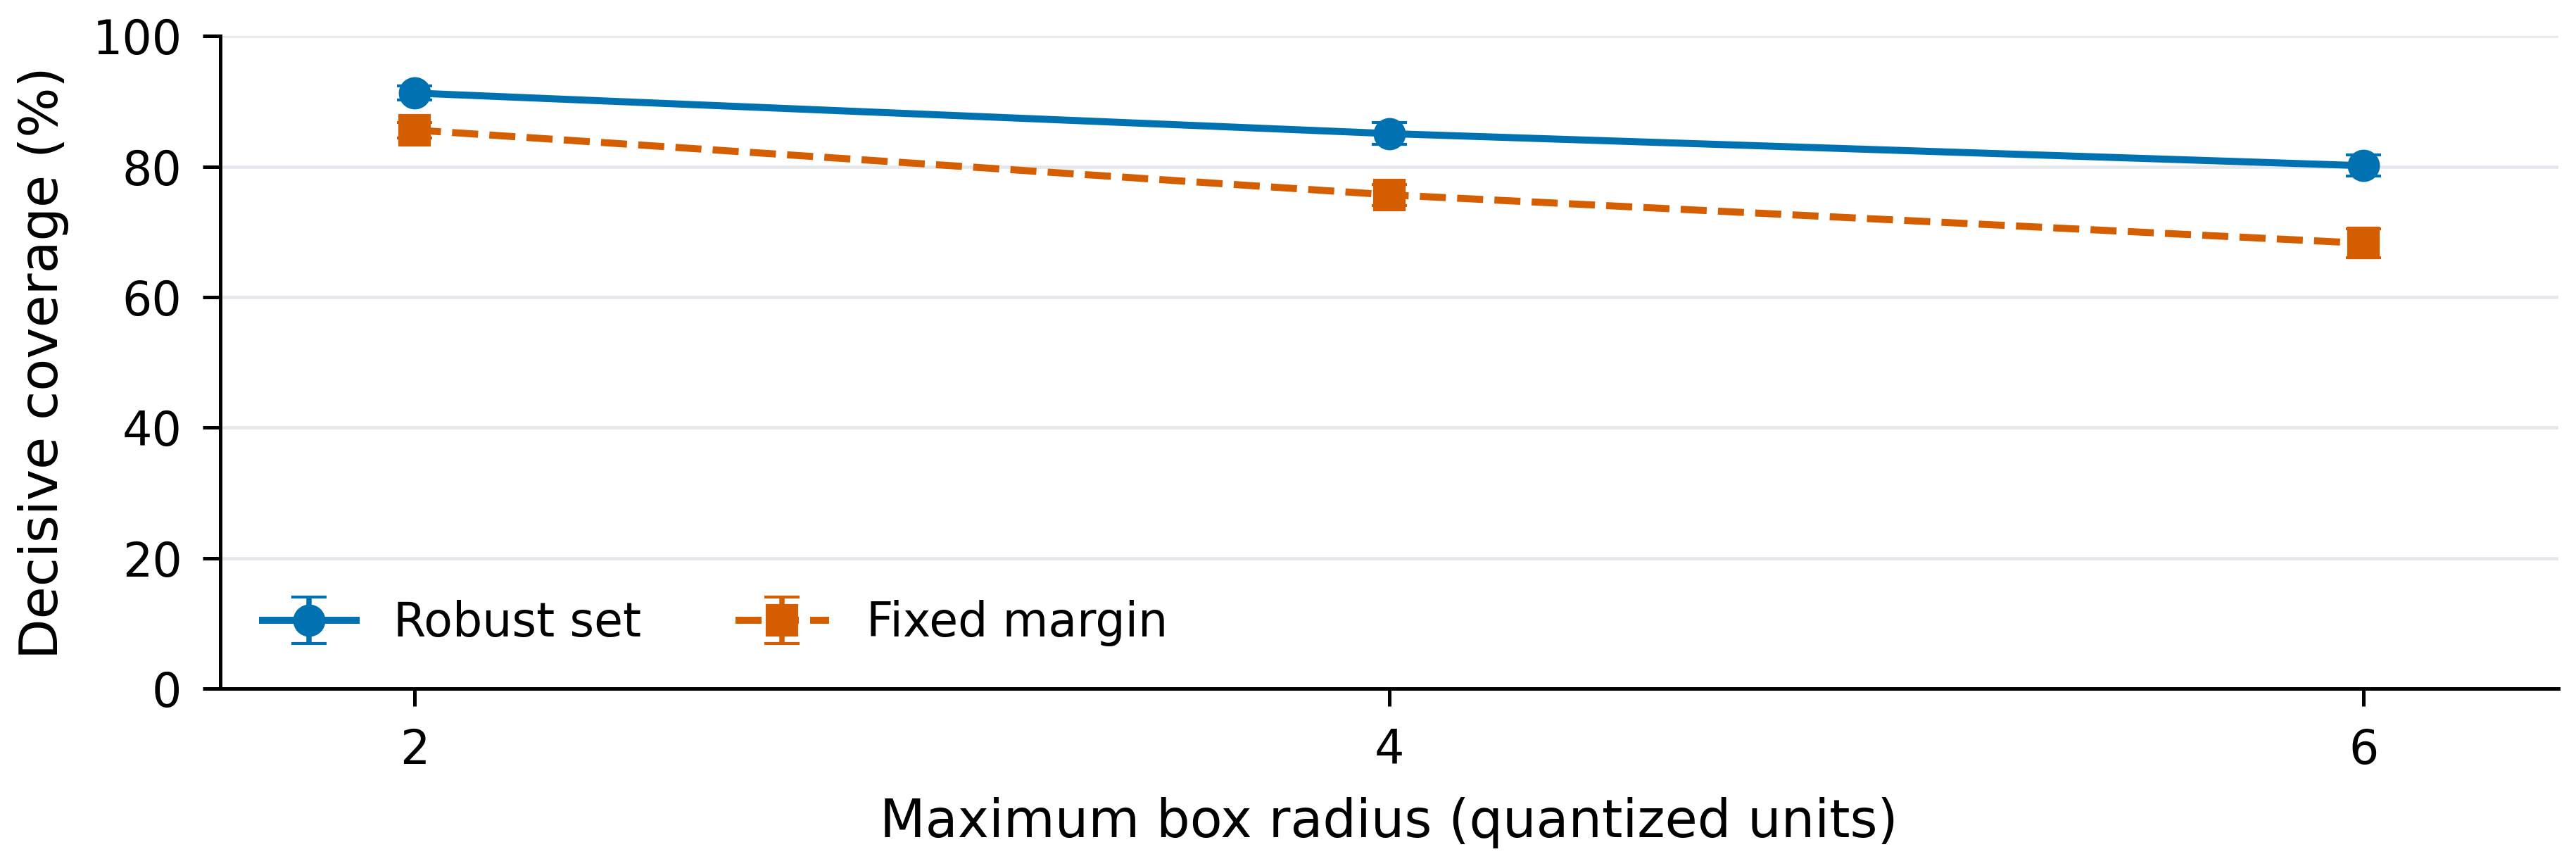
\includegraphics[width=\linewidth]{availability.png}
\caption{Decisive coverage versus maximum uncertainty radius (in quantized units) under correlated calibrated errors with one Byzantine issuer. Error bars denote 95\% confidence intervals across 30 seeds.}\label{fig:availability}
\end{figure}


Figure~\ref{fig:riskcoverage} presents the corresponding risk--coverage operating points for the focus setting. The plotted conditional risk divides wrong decisive outcomes by all decisive classifications, unlike the marginal FA/FR definitions in Table~\ref{tab:semantic}. Since each baseline is tested at one fixed operating point, the figure is an operating-point comparison rather than a continuously tuned risk--coverage curve. For example, all-source intersection achieves only 12.38\% coverage and its 297 decisive decisions are all wrong in the aggregate focus sample; the robust and fixed-margin rules both have zero observed risk at different coverage levels.
\begin{figure}[htbp]\centering
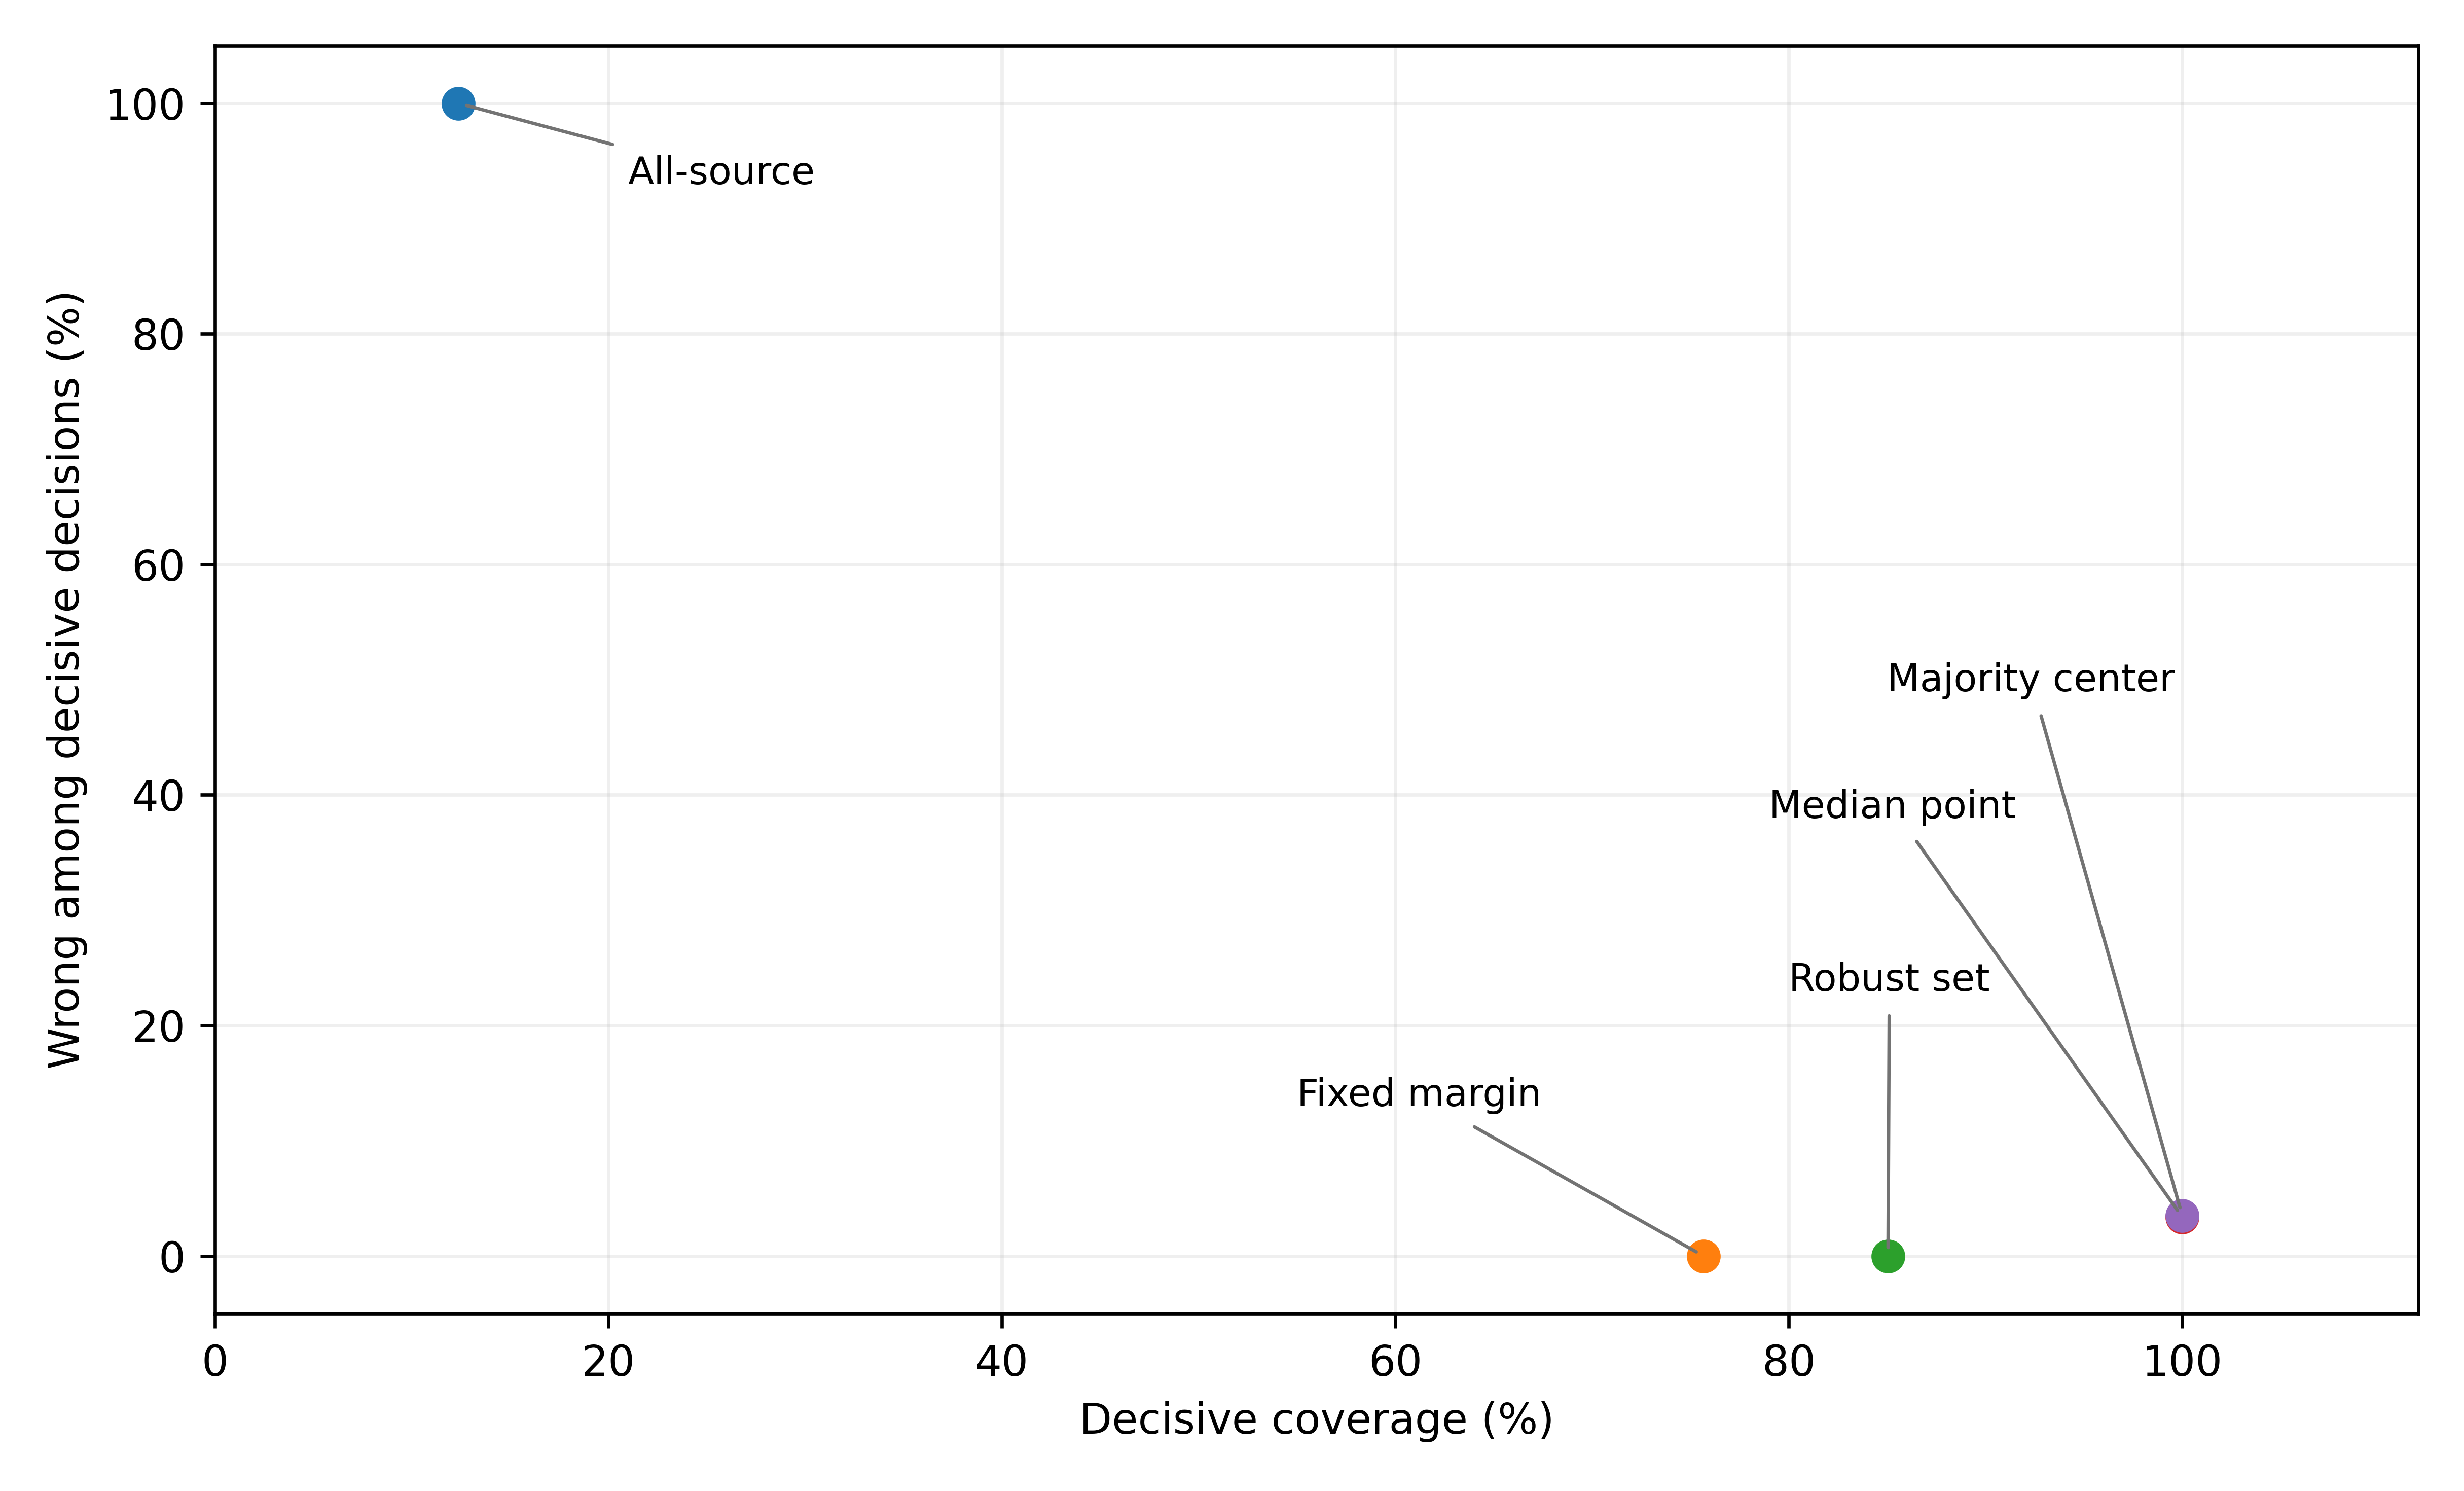
\includegraphics[width=0.92\linewidth]{risk_coverage.png}
\caption{Focus-condition conditional wrong-decision risk versus decisive coverage for five methods; each point uses the aggregate 2,400 generated events. Marginal FA/FR in Table~\ref{tab:semantic} have different denominators.}\label{fig:riskcoverage}
\end{figure}

\subsection{Ablation and out-of-budget stress tests}
Table~\ref{tab:assumption-stress} evaluates system behavior when external assumptions are violated. Under honest-source undercoverage ($M > r$) with one Byzantine issuer, the robust rule experiences 0.23\% FA and 3.41\% FR. When two Byzantine issuers attack a verifier configured for $f = 1$, evidence failure rises to 83.33\% and conditional FA/FR reach 11.62\% and 60.86\%, confirming that the Inconsistent state ($\mathcal{F}_k = \emptyset$) reflects empty threshold support rather than serving as a universal detector for out-of-budget collusion.



\begin{table*}[t]\centering\small
\caption{Stress conditions violating source assumptions: means over 30 seeds (percent).}\label{tab:assumption-stress}
\begin{tabularx}{\linewidth}{@{}Xrrrr@{}}\toprule
Condition&FA&FR&Evidence failure&Decisive\\\midrule
Honest undercoverage; Byzantine count within budget&0.23&3.41&0&84.92\\
Two actual Byzantine issuers with verifier budget $f=1$&11.62&60.86&83.33&16.67\\\bottomrule
\end{tabularx}\end{table*}

Table~\ref{tab:miscoverage} and Figure~\ref{fig:budget} show the paired ablation over the honest-miscoverage budget $r \in \{0, 1, 2\}$ for $n = 5, f = 1$. Because increasing $r$ lowers the support threshold $k = n - f - r$ and expands $\mathcal{F}_k$, it trades decisive coverage for stronger protection against uncalibrated honest misses. Under calibrated evidence, increasing $r$ from 0 to 2 reduces decisive coverage from 85.04\% to 77.46\% while maintaining zero errors. Under undercovered evidence, raising $r$ from 0 to 2 eliminates FA (from 0.23\% to 0\%) and reduces FR from 3.41\% to 0.94\%, with decisive coverage shifting from 84.92\% to 78.50\%.

The UrbanNav trajectory replay shows a similar pattern under simulated multisource errors. Under nominal simulated errors, the robust rule achieves 93.27\% decisive coverage with zero errors, outperforming fixed margins (81.94\%) and avoiding the errors of the median-point baseline (0.29\% FA, 3.12\% FR). Under the $4\times$ common-mode bias stress test, the robust rule maintains low error rates of 0.032\% FA and 0.493\% FR.

\begin{table*}[t]\centering\small
\caption{Paired ablation over honest-miscoverage allowance ($n=5$, $f=1$, maximum radius four, one Byzantine issuer; percent).}\label{tab:miscoverage}
\begin{tabular}{lrrrr}\toprule
Error model&$r$&FA&FR&Decisive coverage\\\midrule
Calibrated&0&0&0&85.04\\
Calibrated&1&0&0&81.25\\
Calibrated&2&0&0&77.46\\
Undercovered&0&0.23&3.41&84.92\\
Undercovered&1&0&1.79&81.67\\
Undercovered&2&0&0.94&78.50\\\bottomrule
\end{tabular}\end{table*}

\begin{figure}[htbp]\centering
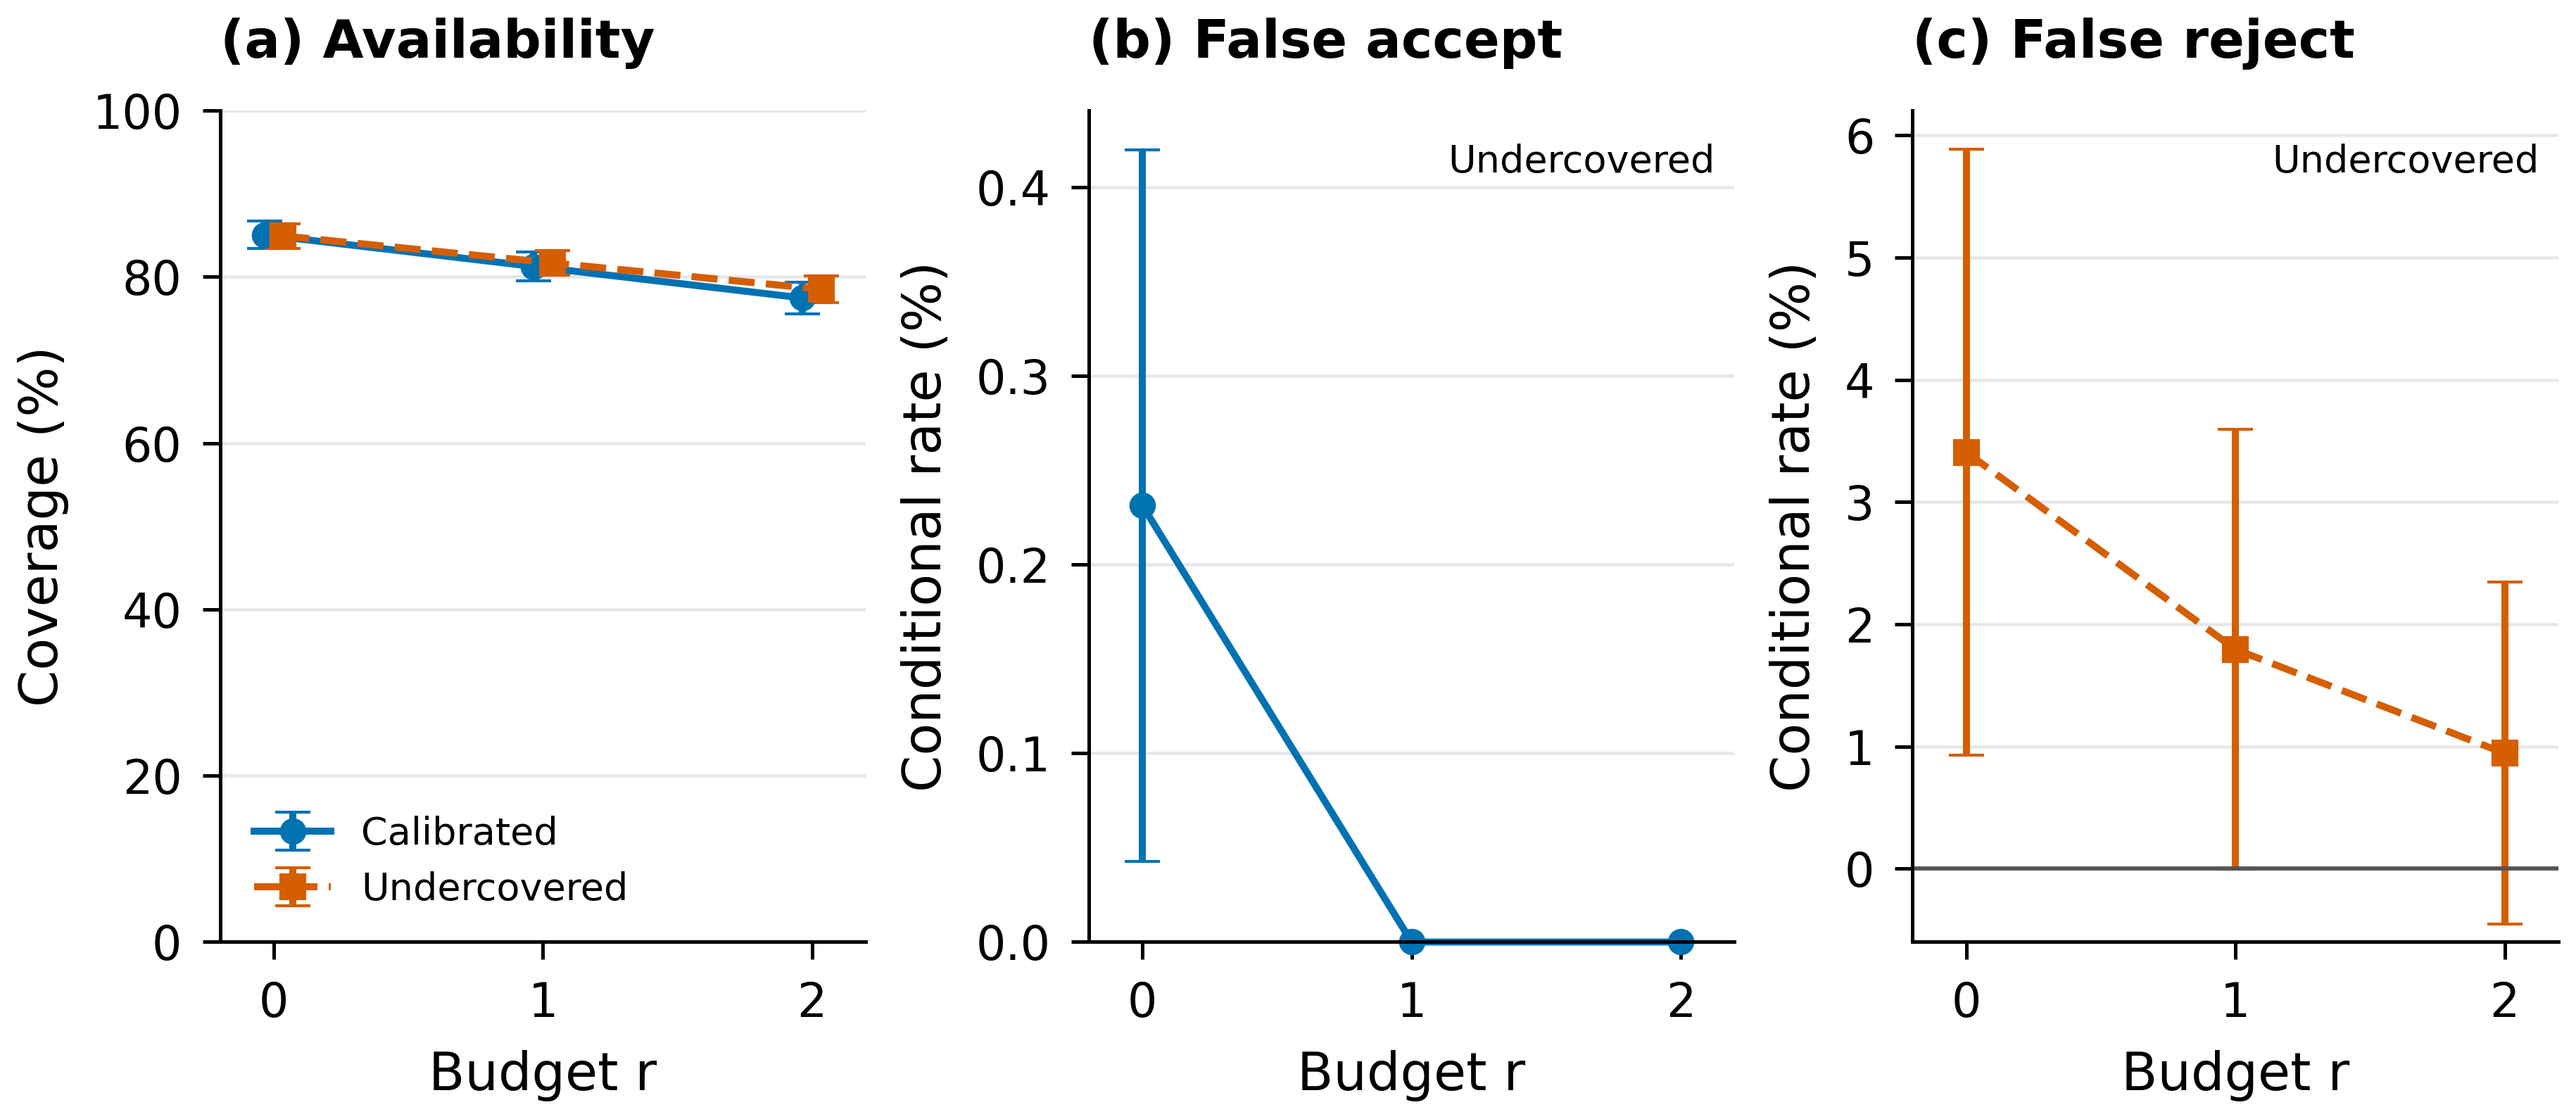
\includegraphics[width=\linewidth]{budget_tradeoff.png}
\caption{Paired ablation over the honest-miscoverage allowance $r$ for $n = 5, f = 1$: (a) decisive coverage, (b) conditional false acceptance, and (c) conditional false rejection. Points represent means and error bars indicate normal-approximation 95\% confidence intervals across 30 seeds.}\label{fig:budget}
\end{figure}
\subsection{Comparison with recent related work}
Table~\ref{tab:recent-context} contextualizes our system alongside recent privacy-preserving localization and Byzantine-tolerant fusion schemes (2024--2026). Because these systems target distinct cryptographic relations and interaction models, Table~\ref{tab:recent-context} highlights their methodological scope alongside reported performance.



\begin{table*}[t]\centering\footnotesize
\caption{Selected quantitative findings from recent systems and the boundaries of comparison. Values are reported by the cited sources.}\label{tab:recent-context}
\begin{tabularx}{\linewidth}{@{}p{0.17\linewidth}p{0.24\linewidth}X@{}}\toprule
Method&Evaluation scale&Reported outcome and methodological boundary\\\midrule
BFT-PoLoc (2024)~\citep{BFTPoLoc}&Up to 450 challengers&At 450 challengers, localization uncertainty was below 100 km for about 45\% of honest targets and below 1000 km for about 95\% of targets; Byzantine network localization rather than a zero-knowledge policy proof\\
PG (2024)~\citep{PG}&261 cloud sensors; 19 constrained sensors&Private Byzantine-tolerant fusion using distributed garbled circuits, with an output-delivery guarantee\\
ZKLP (2025)~\citep{ZKLP}&Floating-point location SNARK&Proximity proof about 0.26 s and verification throughput about 470 peers/s; geometric properties of a hidden point\\
Vehicle ZK-PoL (2025)~\citep{VehiclePolicy}&Up to 43,800 trajectory points&Electric-vehicle subsidy and highway compliance proofs about 36 min and 59 min; interactive, trajectory-scale setting\\
CRSF (2026)~\citep{CRSF}&Up to 261 sensors&At 261 sensors, total measured phase wall time ranged from 0.80 to 1.55 s across reported circuits and scenarios; collusion-resistant private fusion rather than a policy certificate\\\bottomrule
\end{tabularx}
\end{table*}

To provide a direct hardware-normalized reference, we executed the open-source ZKLP implementation (\citet{ZKLP}, pinned at commit \texttt{e8e321524982} using \texttt{gnark} v0.9.1) and our $(n, d) = (3, 2)$ subset circuit (\texttt{gnark} v0.14.0) on the same GitHub Actions Ubuntu runner over 10 post-setup Groth16/BN254 runs. As shown in Table~\ref{tab:zklp-repro}, ZKLP32 compiles to 19,467 constraints with a 515.53 ms median proving time for single-point floating-point proximity. Our $(3, 2)$ subset circuit requires 32,474 constraints and 645.14 ms median proving time, reflecting the additional in-circuit overhead of verifying three EdDSA/MiMC signatures, roster distinctness, context binding, and set-level four-valued reachability while maintaining a compact 164-byte proof and 1.547 ms verification time.

\begin{table*}[t]\centering\footnotesize
\caption{Fixed-version ZKLP reproduction and subset circuit on the same runner (sample medians over ten post-setup proofs).}\label{tab:zklp-repro}
\setlength{\tabcolsep}{3pt}
\begin{tabularx}{\linewidth}{@{}Xrrrrr@{}}\toprule
Implementation&Constraints&Prove (ms)&Verify (ms)&Proof (B)&Public witness (B)\\\midrule
Pinned ZKLP32&19,467&515.53&1.739&196&140\\
Our subset $(3,2)$&32,474&645.14&1.547&164&556\\\bottomrule
\end{tabularx}
\end{table*}

\subsection{Cryptographic performance and circuit scalability}\label{sec:crypto-perf}
\subsubsection{Structural reference using a simplified relation}
Table~\ref{tab:point-zk} reports the baseline overhead of a simplified hidden-point membership circuit on the same Groth16/BN254 stack, which checks only whether a single 16-bit coordinate point lies within $P$. It requires just 408 constraints in 2D and 612 constraints in 3D. In contrast, our full $(3, 2)$ and $(3, 3)$ subset circuits require 32,474 and 35,248 constraints, respectively, demonstrating that in-circuit EdDSA/MiMC signature verification, roster distinctness checks, and context binding dominate the base constraint count in small configurations. Across all configurations, the Groth16 proof size remains constant at 164 bytes.

\begin{table*}[t]\centering\small
\caption{Simplified hidden-point membership circuit with 16-bit bounds under Groth16/BN254.}\label{tab:point-zk}
\begin{tabular}{rrrr}\toprule
Dimension $d$&R1CS constraints&Proof (B)&Public witness (B)\\\midrule
2&408&164&268\\
3&612&164&396\\\bottomrule
\end{tabular}
\end{table*}

\subsubsection{Measured costs of the two geometric backends}
Tables~\ref{tab:crypto} and~\ref{tab:subset} and Figure~\ref{fig:scaling} compare the lower-corner reachability and threshold-subset enumeration ($k = n - 1$) backends primarily on the Apple M1 platform, where public witness sizes range from 556 to 748 bytes. Subset enumeration yields substantially smaller circuits and faster proving times across all tested small-omission configurations. Notably, at $(n, d) = (4, 3)$, lower-corner reachability requires 510,362 constraints and a median proving time of 1090.95 ms, whereas the subset backend requires only 46,737 constraints and 234.93 ms (a $4.64\times$ reduction in median proving latency), while verification remains near 1 ms for both backends.

\begin{table*}[t]\centering\scriptsize
\setlength{\tabcolsep}{3pt}
\caption{Lower-corner Groth16 measurements on the Apple M1; setup in seconds, proving and verification in milliseconds; proof and public witness in bytes.}\label{tab:crypto}
\begin{tabular}{rrrrrrrrr}\toprule
$(n,d)$&Constraints&Setup&Pr p50&Pr p95&Ve p50&Ve p95&Proof&Witness\\\midrule
$(3,2)$&55,987&3.64&213.12&244.83&1.033&1.350&164&556\\
$(4,2)$&97,493&7.47&360.74&427.17&1.081&1.514&164&620\\
$(5,2)$&158,781&11.56&574.69&700.49&1.073&1.212&164&684\\
$(3,3)$&185,229&13.84&548.33&707.35&1.067&1.412&164&684\\
$(4,3)$&510,362&38.34&1090.95&1212.54&1.093&1.506&164&748\\\bottomrule
\end{tabular}
\end{table*}

\begin{table*}[t]\centering\scriptsize
\setlength{\tabcolsep}{3pt}
\caption{Threshold-subset Groth16 measurements with $k=n-1$: Apple M1 unless marked ($\dagger$, GitHub Actions linux/amd64). Setup in seconds, time in milliseconds, sizes in bytes.}\label{tab:subset}
\begin{tabular}{rrrrrrrrr}\toprule
$(n,d)$&Constraints&Setup&Pr p50&Pr p95&Ve p50&Ve p95&Proof&Witness\\\midrule
$(3,2)$&32,474&1.93&163.42&168.89&1.028&1.193&164&556\\
$(4,2)$&42,918&2.83&225.79&234.12&1.038&1.377&164&620\\
$(5,2)$&53,528&3.04&254.66&266.86&1.051&1.343&164&684\\
$(3,3)$&35,248&2.23&206.34&218.98&1.059&1.296&164&684\\
$(4,3)$&46,737&2.71&234.93&248.10&1.038&1.235&164&748\\
$(8,2)^\dagger$&86,354&10.85&902.09&927.00&1.237&1.438&164&876\\\bottomrule
\end{tabular}
\end{table*}

\begin{figure}[htbp]\centering
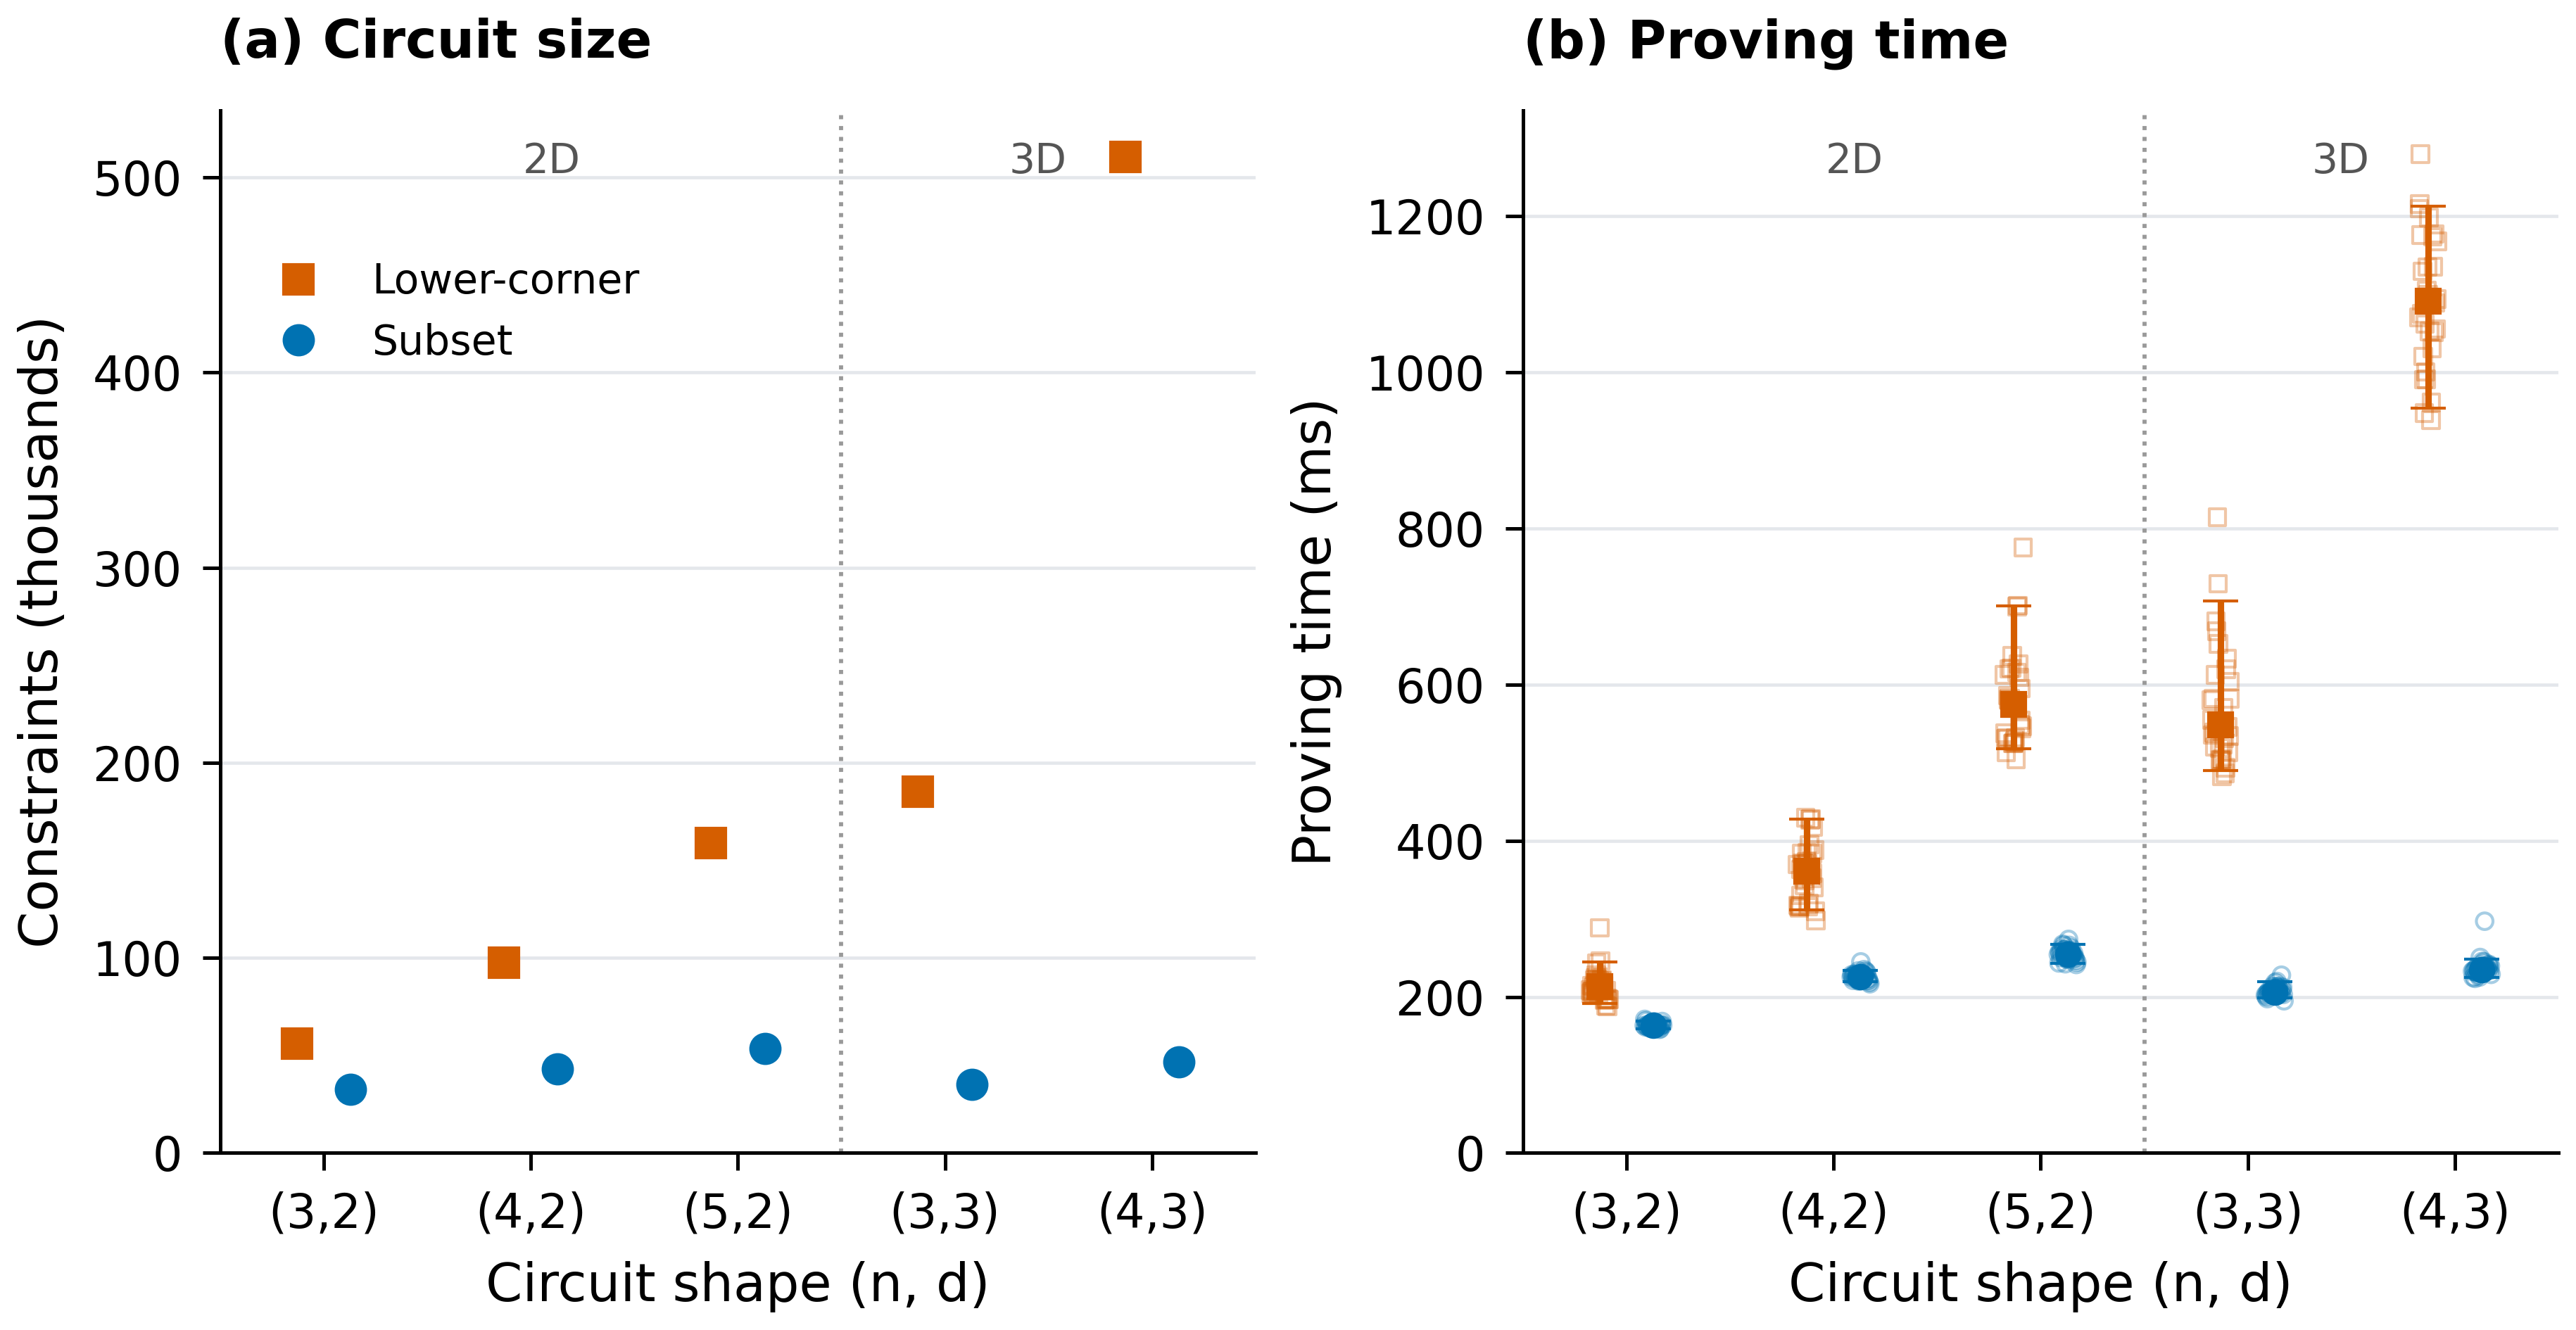
\includegraphics[width=\linewidth]{backend_costs.png}
\caption{R1CS constraint counts (a) and proving times (b) for the lower-corner and subset ($k = n - 1$) backends on the Apple M1 platform. Large markers denote medians, error bars span the empirical p5--p95 range, and light points plot all 30 trials per configuration.}\label{fig:scaling}
\end{figure}

\subsubsection{Resource-limited compilation scalability}
Table~\ref{tab:compilegrowth} and Figure~\ref{fig:compilegrowth} summarize the 32 resource-bounded R1CS compilation runs across $n \in \{4, 8, 12, 16\}$ and $d \in \{2, 3\}$, where 27 runs completed within the 3 GiB RSS / 30 s budget and 5 reached the resource limit (RL). At $(d, n) = (2, 16)$, lower-corner reachability generates 3,509,645 constraints, compared with only 181,194 ($b = 1$) and 308,978 ($b = 2$) for the subset backend. A full end-to-end n=8 subset proof experiment is reported separately below. In 3D ($d = 3$), lower-corner reachability exceeds the 3 GiB compilation limit for $n \ge 8$, whereas subset enumeration with $b \in \{1, 2\}$ compiles within the stated resource budget up to $n = 16$ (203,793 and 395,417 constraints). Conversely, when the omission budget grows to $k = n/2$, combinatorial subset growth becomes apparent, reaching 962,018 constraints at $(d, n, k) = (3, 12, 6)$. These compilation results indicate that threshold-subset enumeration has a substantially smaller constraint footprint for small fault and miscoverage budgets ($b = f + r \ll n$), while lower-corner reachability provides threshold flexibility for small issuer rosters.


\paragraph{Independent eight-issuer proving run.} To distinguish R1CS compilation from actual cryptographic execution, we performed 30 post-setup proofs with $n=8$, $d=2$, and omission budget $b=1$ using the full subset circuit on a GitHub Actions \texttt{linux/amd64} runner (Go 1.25.0, gnark 0.14.0). The circuit contains 86,354 constraints, setup took 10.852 s, proving p50/p95 were 902.089/926.998 ms, verification p50/p95 were 1.237/1.438 ms, the proof was 164 bytes, and the public witness occupied 876 bytes. The 30 runs include Groth16 proof generation and verification; their hardware environment differs from the Apple M1 used for Tables~\ref{tab:crypto}--\ref{tab:subset}. The pinned workflow and machine-readable record are available via the experimental repository and its archived CI run.

\begin{table*}[t]\centering\small
\caption{Resource-limited R1CS compilation sweep with complete signature and geometric constraints. \texttt{RL} indicates termination before a count was obtained.}\label{tab:compilegrowth}
\begin{tabular}{rrrrrr}\toprule
$d$&$n$&Lower corner&Subset $b=1$&Subset $b=2$&Subset $k=n/2$\\\midrule
2&4&97,493&42,918&43,160&43,160\\
2&8&509,277&86,354&97,734&111,776\\
2&12&1,544,390&132,447&181,221&675,759\\
2&16&3,509,645&181,194&308,978&RL\\
3&4&510,362&46,737&47,099&47,099\\
3&8&RL&95,153&112,213&133,255\\
3&12&RL&147,506&220,640&962,018\\
3&16&RL&203,793&395,417&RL\\\bottomrule
\end{tabular}\end{table*}

\begin{figure}[htbp]\centering
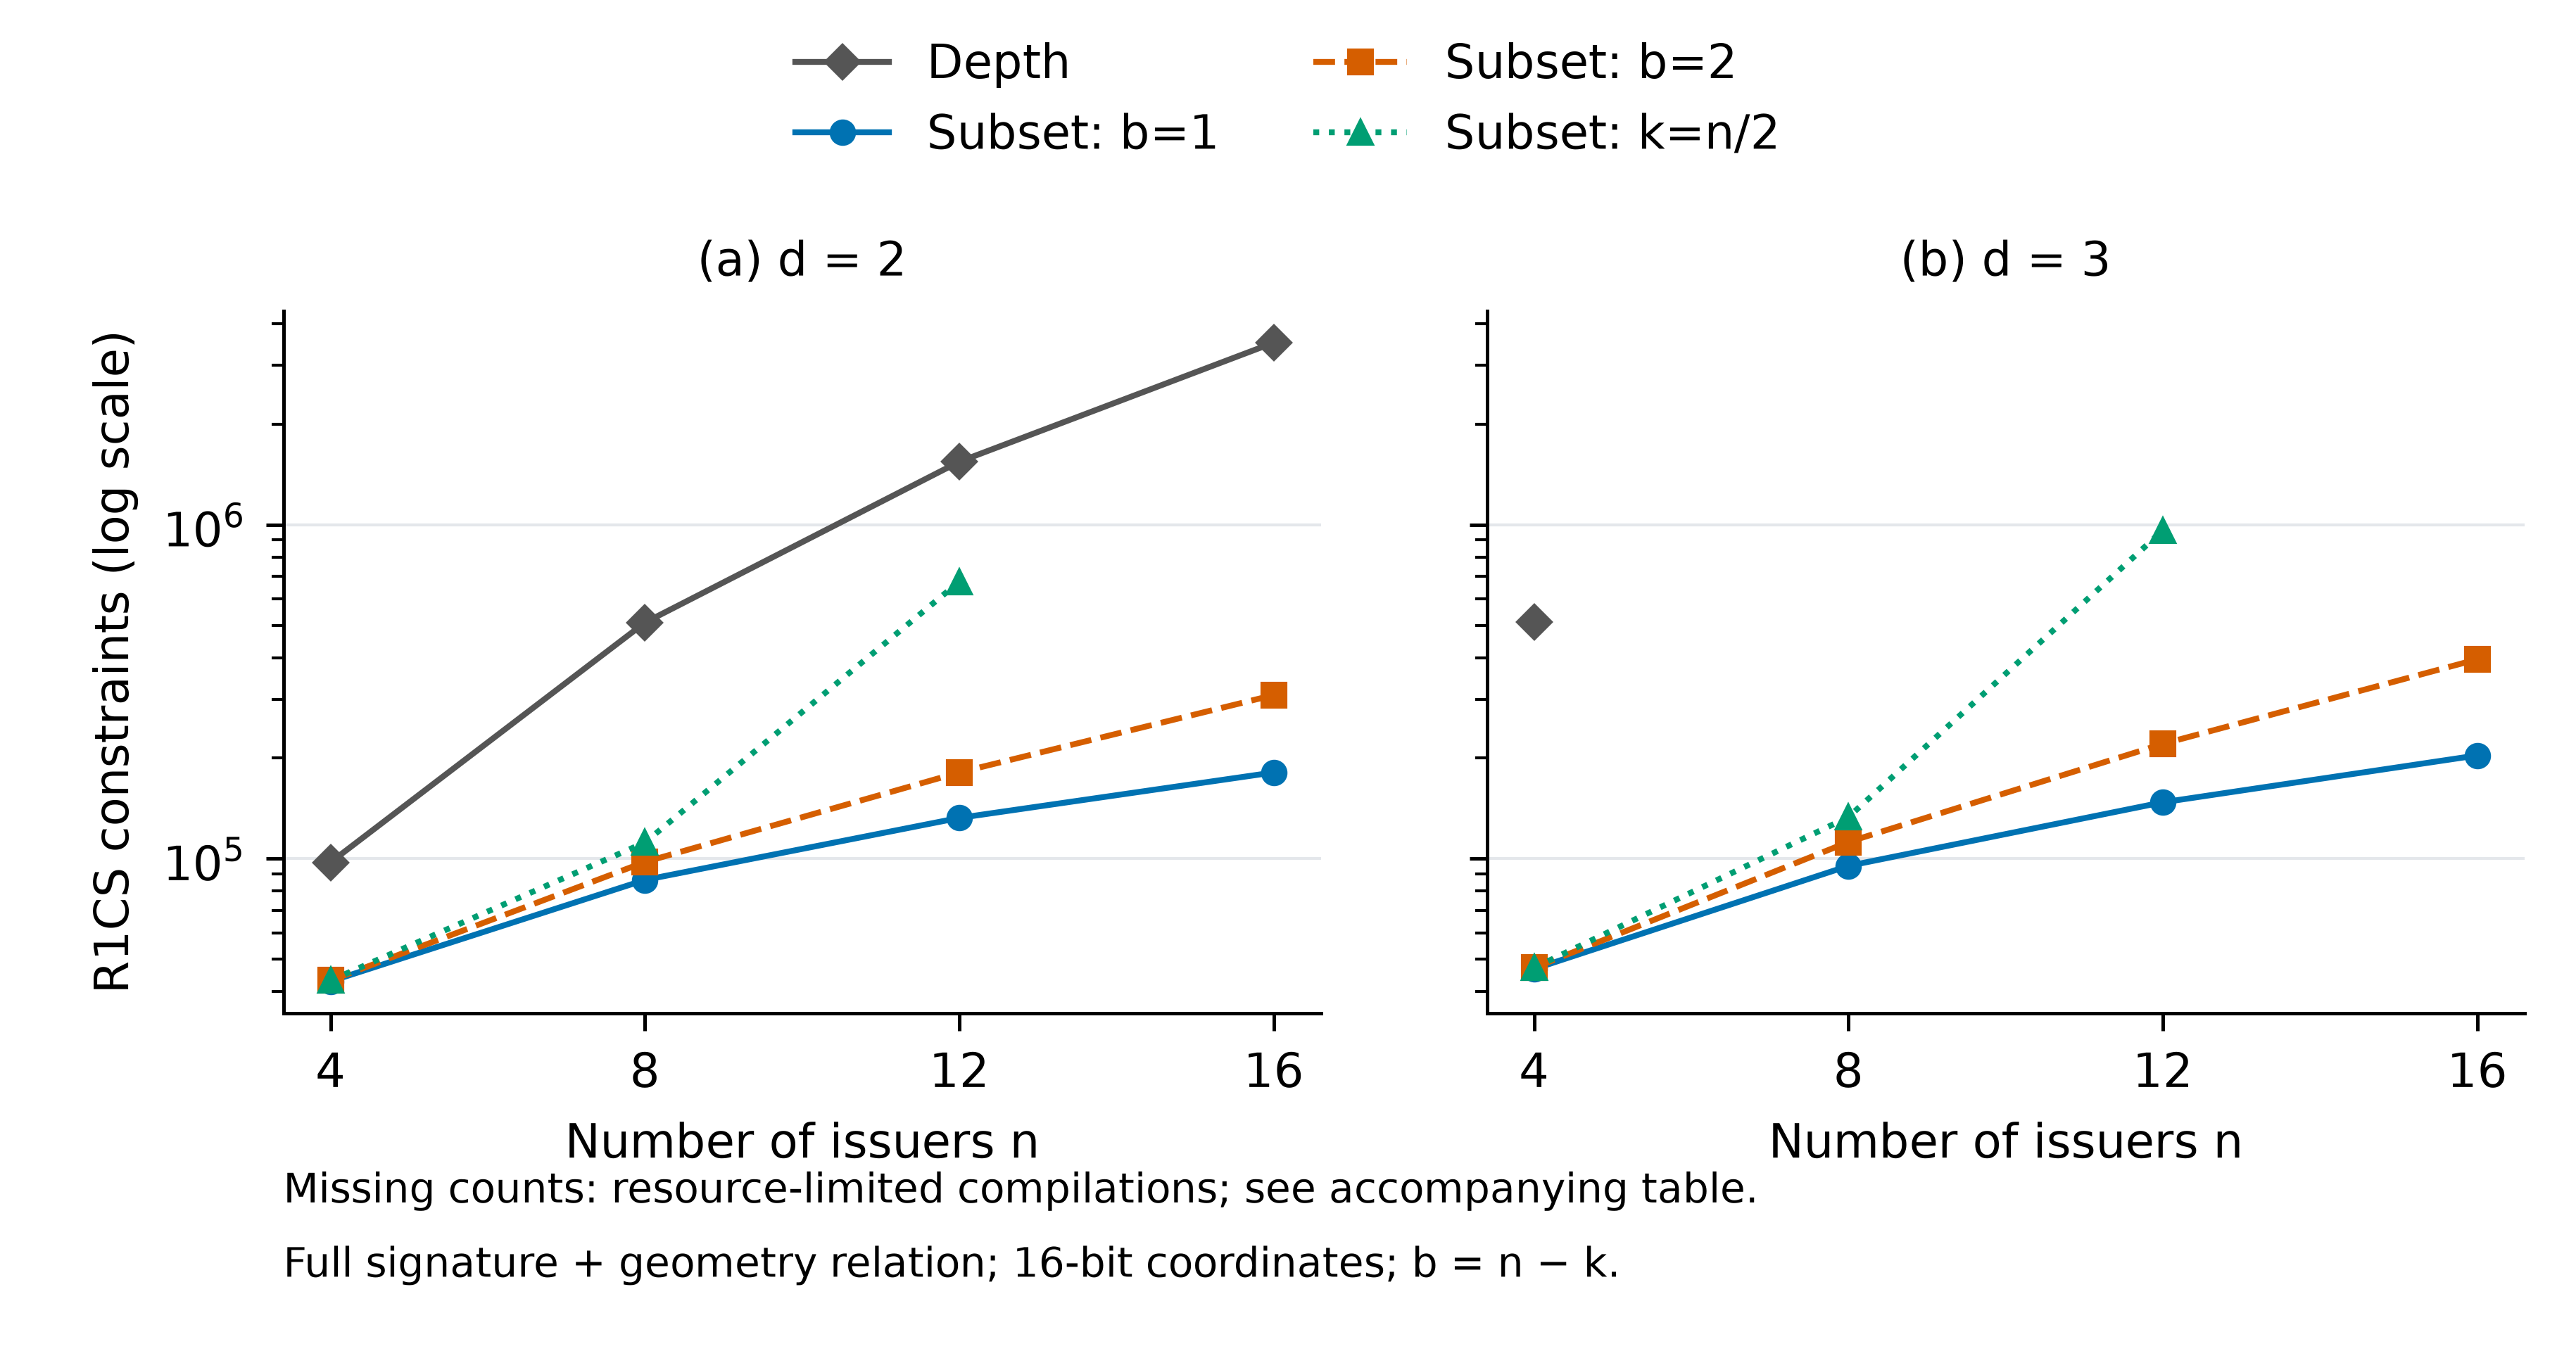
\includegraphics[width=\linewidth]{compile_scalability.png}
\caption{R1CS constraint scaling across issuer count $n$ and dimension $d \in \{2, 3\}$ for full signature and geometry circuits under a 3 GiB RSS compilation limit.}\label{fig:compilegrowth}
\end{figure}
\section{Discussion}
The experiments illustrate the interaction between robust evidence fusion and private certification. Across the 12 synthetic conditions satisfying the configured fault and coverage budgets, the feasible-set rule produced no wrong decisive classifications and achieved mean decisive coverage of 87.52\%, compared with 75.63\% for the fixed-margin baseline. The paired ablation also shows how the honest-miscoverage allowance $r$ controls the trade-off between decisive coverage and robustness to undercoverage. These findings complement the conditional soundness argument: the rule retains all states supported by the required number of issuers and certifies compliance only when the resulting set satisfies the policy.

The two exact circuit backends offer different computational trade-offs. Lower-corner reachability accepts a dynamic threshold, while threshold-subset enumeration fixes the threshold at compilation and reduces the constraint count for the small-omission configurations tested. For $(n,d)=(4,3)$, the subset backend reduced the median proving time from 1090.95 ms to 234.93 ms on the Apple M1, with 164-byte proofs in both cases. These measurements reflect complete signed-evidence circuits rather than geometric checks alone.

The proof protects the signed interval witness while binding the classification to the task, roster, report, and challenge. The reported guarantees depend on the stated physical coverage and fault budgets, the fixed roster requires complete evidence, and the report and public outputs remain visible. The prototype uses Groth16/BN254 with gnark's twisted-Edwards EdDSA/MiMC; BN254 provides approximately 100-bit security under contemporary estimates, and its evidence signatures are distinct from IEEE 1609.2-compliant ECDSA credentials.

\section{Conclusion}
The compliance rule considers the set of states supported by at least $k = n - f - r$ signed uncertainty intervals. It returns one of four decisions (Valid, Invalid, Ambiguous, and Inconsistent); a report is accepted only if the feasible set is nonempty and contained within the authorized policy.

The implementation combines two exact Groth16/BN254 circuit backends---lower-corner reachability and threshold-subset enumeration---with a challenge-bound verification gateway. Across 12 calibrated synthetic conditions satisfying the fault and coverage budgets, the robust rule exhibited no wrong decisive classifications in the evaluated within-budget cases while improving mean decisive coverage to 87.52\% over a fixed-margin baseline (75.63\%). For small omission budgets, the subset backend achieves 164-byte proofs and 163--255 ms median proving times on an Apple M1.

\appendix
\section{Retrospective single-receiver calibration diagnostic}\label{app:receiver}
To illustrate how a static uncertainty envelope can degrade across operating periods, we conduct a retrospective diagnostic on the TST2 reference sequence from GraphGNSSLib ~\citep{GraphGNSSData}, which comprises 157 matched epochs of precomputed RTKLIB 2.4.2 kinematic combined solutions. Horizontal east ($e_j$) and north ($n_j$) residuals are computed relative to the ground-truth reference coordinates.

We reserve the first 78 chronological epochs for calibration, leave a 10-epoch gap, and evaluate the final 69 epochs. Defining the Chebyshev residual $s_j = \max(\vert{}e_j\vert{}, \vert{}n_j\vert{})$, the 76th ordered calibration score yields an axis-aligned square envelope of half-width $0.863506\text{ m}$. We compare this empirical square against the solution-reported $3\sigma$ rectangular envelope in Table~\ref{tab:receiver}.

\begin{table*}[t]\centering\small
\caption{Reference-position containment in the single-receiver diagnostic (contained epochs / available epochs). Temporal epochs are not independent trials.}\label{tab:receiver}
\begin{tabularx}{\linewidth}{@{}Xrr@{}}\toprule
Envelope rule&Calibration (78)&Evaluation (69)\\\midrule
Solution-reported $3\sigma$ rectangle&8/78&0/69\\
Empirically calibrated square (0.863506 m half-width)&76/78&2/69\\\bottomrule
\end{tabularx}
\end{table*}

While the empirically calibrated square encloses 76/78 reference positions during the calibration window, it covers only 2/69 positions in the evaluation window (and the reported $3\sigma$ rectangle covers 8/78 and 0/69, respectively), as the median horizontal residual drifts from $0.869\text{ m}$ to $1.038\text{ m}$ (Figure~\ref{fig:receiver}). The observed drift illustrates the role of the physical coverage premise ($M \le r$) in Section 4.

\begin{figure}[htbp]\centering
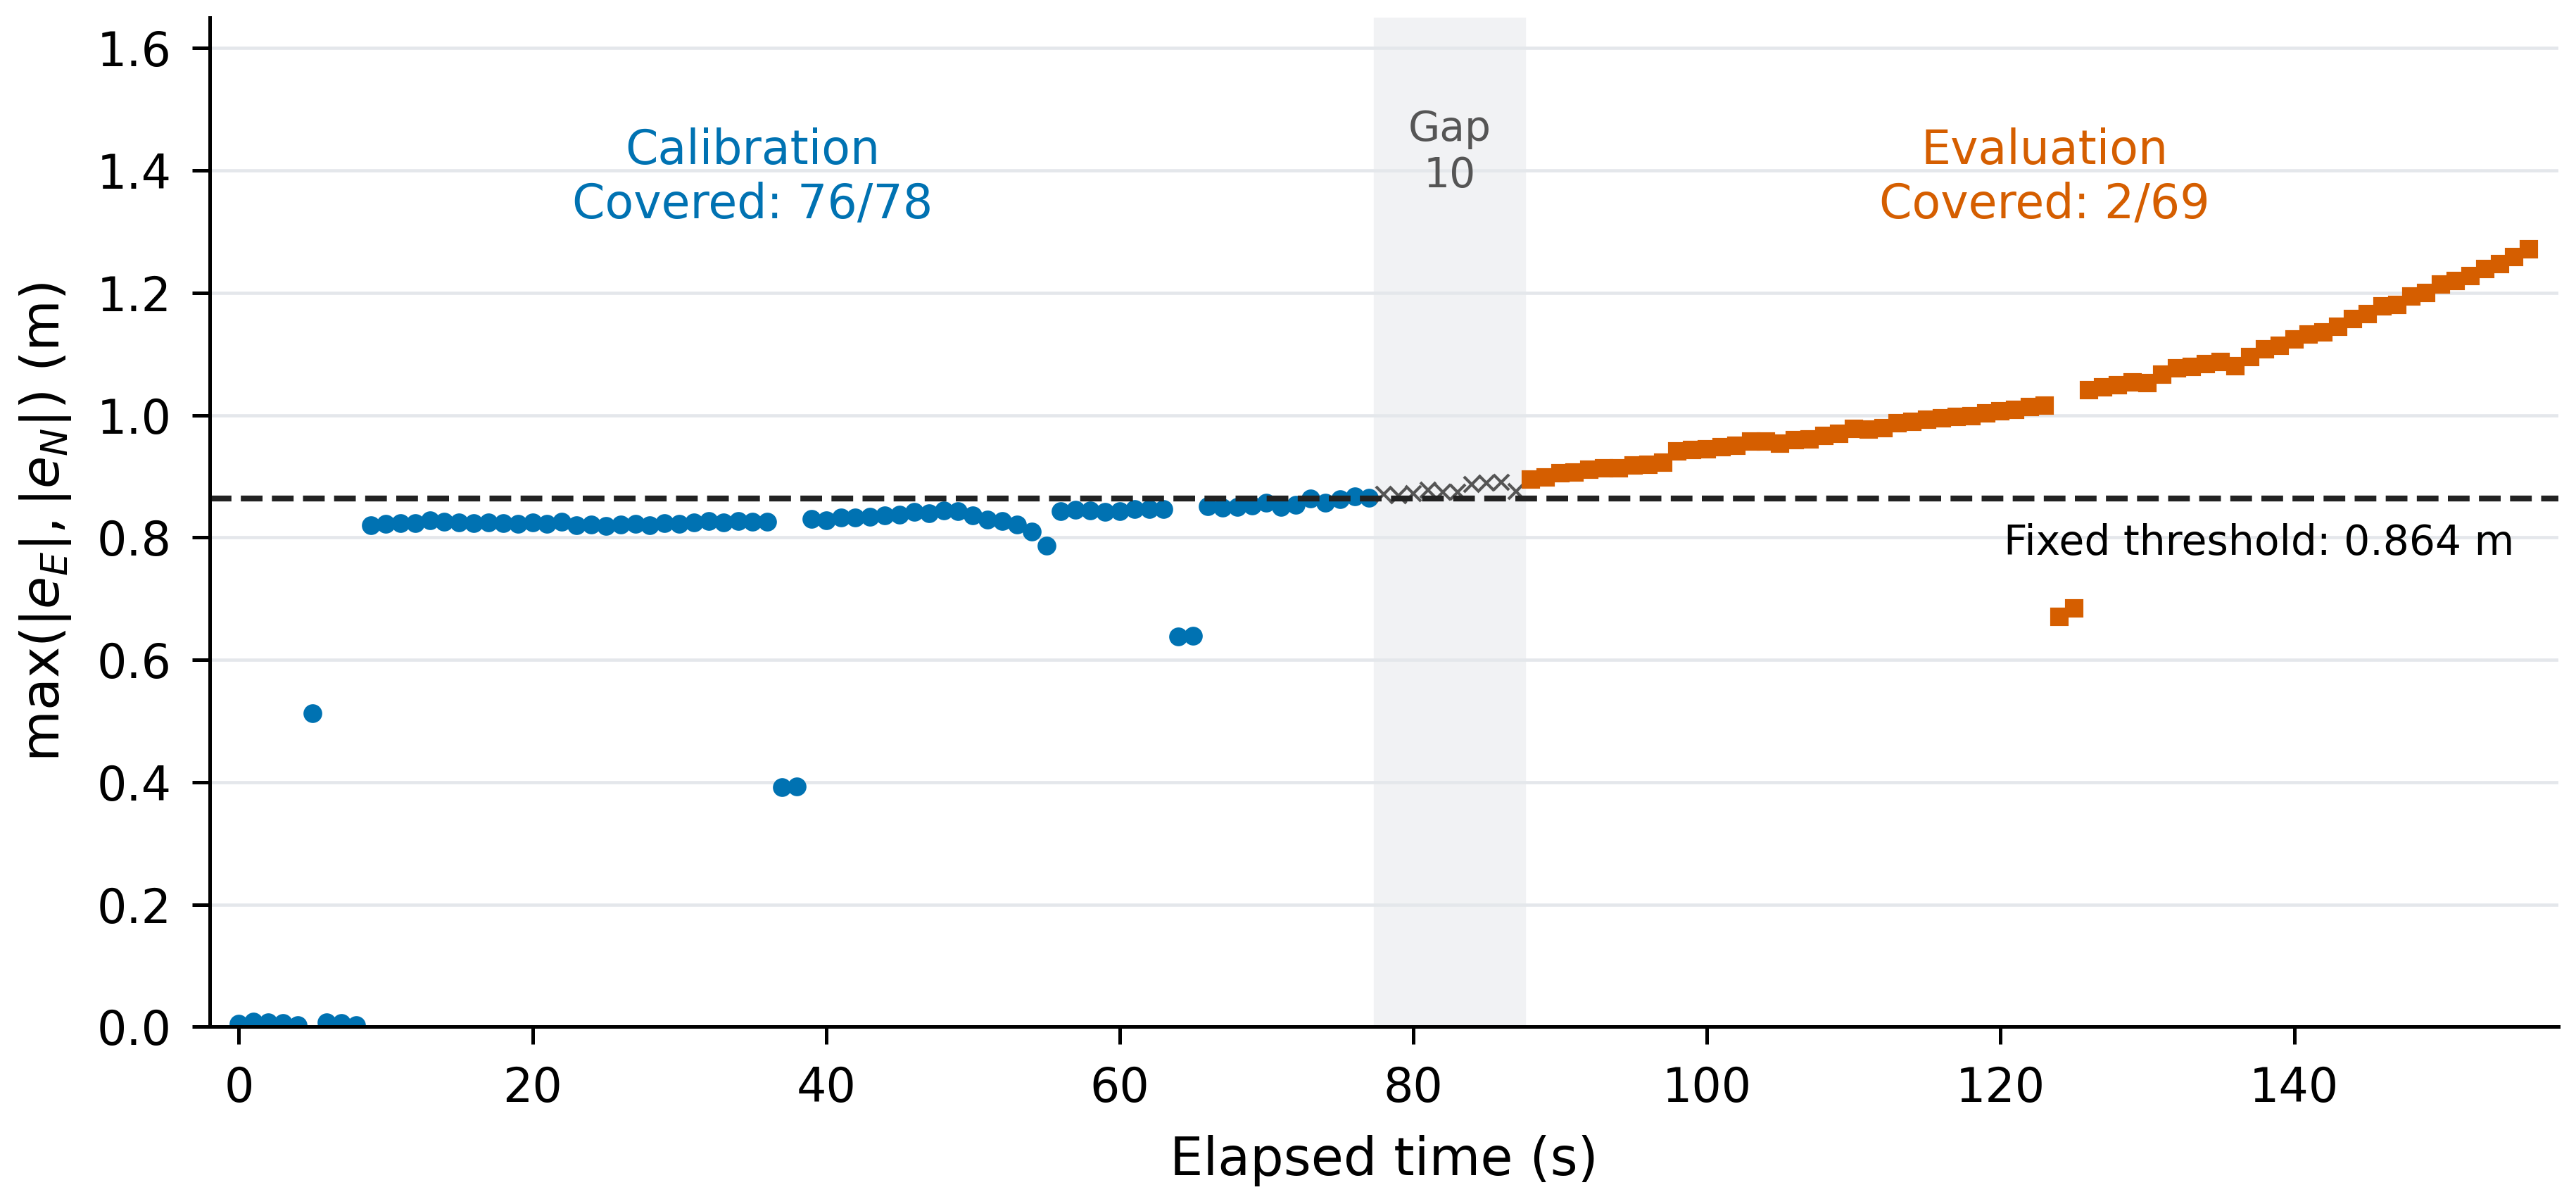
\includegraphics[width=\linewidth]{receiver_diagnostic.png}
\caption{Horizontal Chebyshev residual trajectory ($\max(|e_E|, |e_N|)$) across 157 stationary epochs, illustrating how a fixed $0.864\text{ m}$ calibration threshold fails to cover subsequent drift in the evaluation window.}\label{fig:receiver}
\end{figure}

\bibliography{references}
\section*{Statements and Declarations}
\noindent\textbf{Funding:} This study received partial support from the Heilongjiang Provincial University Teacher Scientific Research Business Fee (2018-KYYWF0941), the Heilongjiang Provincial Natural Science Foundation Joint Fund Cultivation Project (PL2024F002), the National Foreign Expert Key Support Project (D2O25O185), and the Heilongjiang Provincial Undergraduate University Excellent Young Teacher Fundamental Research Support Plan (YQJH2024239).

\noindent\textbf{Competing interests:} The authors declare that they have no known competing financial interests or personal relationships that could have appeared to influence the work reported in this paper.

\noindent\textbf{Author contributions:} Lili He: supervision. Sheng Jiang: methodology, software, investigation, formal analysis. Shuang Chen: writing -- original draft. Lei Zhang: supervision, corresponding author.

\noindent\textbf{Data and code availability:} The proof prototype, synthetic evaluations, benchmark logs, and reproducibility records are available at \url{https://github.com/js110/ZCRSC-PAPER}.

\end{document}
